%%%%%%%%%%%%%%%%%%%%%%%%%%%%%%%%%%%%%%%%%%%%%%%%%%%%%%%%%%%%%%%%%%%%%%%%%%%%
%% Author template for INFORMS Journal on Computing (ijoc)
%% Mirko Janc, Ph.D., INFORMS, mirko.janc@informs.org
%% ver. 0.95, December 2010
%%%%%%%%%%%%%%%%%%%%%%%%%%%%%%%%%%%%%%%%%%%%%%%%%%%%%%%%%%%%%%%%%%%%%%%%%%%%
%\documentclass[ijoc,blindrev]{informs3}
\documentclass[ijoc,nonblindrev]{informs3} % current default for manuscript submission
%\documentclass[dvips,ijoc]{informs3}      % if dvips is used
%\documentclass[dvipsone,ijoc]{informs3}   % if dvipsone is used, etc.

%%\OneAndAHalfSpacedXI
\OneAndAHalfSpacedXII % current default line spacing
%%\DoubleSpacedXII
%%\DoubleSpacedXI

% If hyperref is used, dvi-to-ps driver of choice must be declared as
%   an additional option to the \documentclass. For example
%\documentclass[dvips,ijoc]{informs3}      % if dvips is used
%\documentclass[dvipsone,ijoc]{informs3}   % if dvipsone is used, etc.

% Private macros here (check that there is no clash with the style)

% Natbib setup for author-year style
\usepackage{natbib}
 \bibpunct[, ]{(}{)}{,}{a}{}{,}%
 \def\bibfont{\small}%
 \def\bibsep{\smallskipamount}%
 \def\bibhang{24pt}%
 \def\newblock{\ }%
 \def\BIBand{and}%
 
\usepackage{array}
\usepackage{multirow}
\usepackage{hyperref}
\usepackage{tabto}
\usepackage{tikz}
\usepackage{graphicx,wrapfig,lipsum}
\usepackage{booktabs}
%\usepackage{graphicx}
%\usepackage[colorlinks=true,citecolor=black,linkcolor=black,urlcolor=blue]{hyperref}
\usepackage{graphics,color,float,epsf,caption,subcaption}
\usepackage{enumerate}
\usepackage{amsmath}
\usepackage{amssymb}
\numberwithin{equation}{subsection}
\usepackage{algorithm,algorithmic}
\usepackage{float}

%% Setup of theorem styles. Outcomment only one. 
%% Preferred default is the first option.
\TheoremsNumberedThrough     % Preferred (Theorem 1, Lemma 1, Theorem 2)
%\TheoremsNumberedByChapter  % (Theorem 1.1, Lema 1.1, Theorem 1.2)

%% Setup of the equation numbering system. Outcomment only one.
%% Preferred default is the first option.
\EquationsNumberedThrough    % Default: (1), (2), ...
%\EquationsNumberedBySection % (1.1), (1.2), ...

% In the reviewing and copyediting stage enter the manuscript number.
\MANUSCRIPTNO{XXXX} % When the article is logged in and DOI assigned to it,
                 %   this manuscript number is no longer necessary

%%%%%%%%%%%%%%%%
\begin{document}
%%%%%%%%%%%%%%%%

% Outcomment only when entries are known. Otherwise leave as is and 
%   default values will be used.
%\setcounter{page}{1}
%\VOLUME{00}%
%\NO{0}%
%\MONTH{Xxxxx}% (month or a similar seasonal id)
%\YEAR{0000}% e.g., 2005
%\FIRSTPAGE{000}%
%\LASTPAGE{000}%
%\SHORTYEAR{00}% shortened year (two-digit)
%\ISSUE{0000} %
%\LONGFIRSTPAGE{0001} %
%\DOI{10.1287/xxxx.0000.0000}%

% Author's names for the running heads
% Sample depending on the number of authors;
% \RUNAUTHOR{Jones}
% \RUNAUTHOR{Jones and Wilson}
% \RUNAUTHOR{Jones, Miller, and Wilson}
% \RUNAUTHOR{Jones et al.} % for four or more authors
% Enter authors following the given pattern:
\RUNAUTHOR{Ferdman, Minkov, and Bekkerman}

% Title or shortened title suitable for running heads. Sample:
% \RUNTITLE{Bundling Information Goods of Decreasing Value}
% Enter the (shortened) title:
\RUNTITLE{The ecology of the Web browser}

% Full title. Sample:
\TITLE{The ecology of the Web browser}
% The ecology of the Web browser
%\TITLE{}

% Block of authors and their affiliations starts here:
% NOTE: Authors with same affiliation, if the order of authors allows, 
%   should be entered in ONE field, separated by a comma. 
%   \EMAIL field can be repeated if more than one author
\ARTICLEAUTHORS{%
\AUTHOR{Sela Ferdman}
\AFF{University of Haifa, \EMAIL{sela.ferdman@gmail.com}}
\AUTHOR{Einat Minkov}
\AFF{University of Haifa, \EMAIL{einatm@is.haifa.ac.il}}
\AUTHOR{Ron Bekkerman}
\AFF{University of Haifa, \EMAIL{ronb@univ.haifa.ac.il}}
% Enter all authors
} % end of the block

\ABSTRACT{%

The question ``How do intelligent machines coexist with humans?'' has recently received a new wave of attention. In this paper, we deal with the question ``How do machines coexist with each other?''. While the human-machine interaction has been in the focus of the research community for decades, the machine-machine interaction has been largely overlooked in the literature. The general assumption has so far been that machines are supposed to cooperate for the human's good, but it is not always the case. We claim that machines and humans comprise a complex ecosystem and show that \emph{ecology} is a feasible framework for modeling  processes in the new world where machines are no longer under the full control of humans. We do so over a case study of Web browser's \emph{addons} --- a domain in which ``machines'' (i.e.~addons) have been coexisting for years. 

The Web browser is the user's window to the World Wide Web. All Web browsers extend their
offerings via browser addons. There is an enormous amount of various addons available on the Web.
The decision whether to install a particular addon is usually in the user's hands, so that the set of addons
installed on the user's machine partially reflects the user's preferences, interests, and behavioral characteristics. 

Not all decisions about installing or removing addons are up to the user. Some addons ``sneak in''
the user's machine via third party installations, while some installed addons ``kick out'' their competitors
without the user's involvement. Most often, these processes follow business decisions of addon manufacturing
companies that engage in partnerships with each other or compete over the user's attention.
Users with their personal preferences and addon companies with their business goals make the Web browser a
complex ecosystem which we study in this paper.

Our research goals are two fold. First, we investigate the Web browser ecosystem at the micro-level,
i.e.~at the level of an individual user's machine. We empirically show that the Web browser ecosystem
bears characteristics of a biological ecosystem. Provided with a unique dataset of addons installed on
almost a million of real users' machines, we construct a large-scale graph with nodes corresponding to
users, addons, and words (terms) extracted from the addons' attributes. We use the Personalized PageRank (PPR)
random walk to traverse the graph and confirm the \emph{ecological resilience} of the individual Web browser ecosystem. We
show that our PPR-based model significantly outperforms non-personalized models in detecting the resilience.

Next, we adapt our PPR-based model to
analyzing the Web browser ecosystem at the macro-level, i.e. at the level of addon manufacturers involved
in business activities. We hypothesize that some addon companies live in \emph{symbiosis} or \emph{clash} with each
other. In our large-scale dataset of addons, we identify nineteen prominent addon manufacturers and use the adapted PPR-based model to detect symbiotic and clash relationships between some of
the nineteen companies. We partly validate our results in online media, while the rest of them shed
light on well hidden relationships within the Web browser ecosystem. By showing the direct connection between biological and digital ecosystems, our work invites ecologists to apply their methodologies to studying the new bio-digital ecology.
}%

% Sample 
%\KEYWORDS{deterministic inventory theory; infinite linear programming duality; 
%  existence of optimal policies; semi-Markov decision process; cyclic schedule}

% Fill in data. If unknown, outcomment the field
\KEYWORDS{personalized pagerank, ecosystem}
\HISTORY{}

\maketitle
%%%%%%%%%%%%%%%%%%%%%%%%%%%%%%%%%%%%%%%%%%%%%%%%%%%%%%%%%%%%%%%%%%%%%%

% Samples of sectioning (and labeling) in IJOC
% NOTE: (1) \section and \subsection do NOT end with a period
%       (2) \subsubsection and lower need end punctuation
%       (3) capitalization is as shown (title style).
%
%\section{Introduction.}\label{intro} %%1.
%\subsection{Duality and the Classical EOQ Problem.}\label{class-EOQ} %% 1.1.
%\subsection{Outline.}\label{outline1} %% 1.2.
%\subsubsection{Cyclic Schedules for the General Deterministic SMDP.}
%  \label{cyclic-schedules} %% 1.2.1
%\section{Problem Description.}\label{problemdescription} %% 2.

% Text of your paper here
\newpage
\section {Introduction}
\pagenumbering{arabic}

With the dramatic developments in AI technologies over the past 5 years, questions traditionally discussed in science fiction literature have recently been brought to the spotlight of public attention. In their seminal paper, \cite{russell2016research} posed some of those questions, mostly related to the legal, ethical, and structural regulation of decisions that can be made by intelligent systems. The paper led to formulating a widely recognized Open Letter on research priorities for robust and beneficial AI, signed so far by over 8000 scientists and technologists (including Stephen Hawking, Bill Gates, Elon Musk, and many other top influencers). The goal of the open letter is clear: ``our AI systems must do what we want them to do''. What is less clear, however, is how this goal can be achieved. \cite{amodei2016concrete} went much further into practical aspects of achieving this goal: they proposed concrete methods for minimizing damage that an intelligent system may cause to its environment. While Amodei et al.'s paper paves a way to building harmless AI, it makes it apparent that not all possible problems can be identified and immediately solved. The world in which both humans and machines are first-class citizens is much more complex than we could have imagined.

A lot has been said about coexistence of humans and machines, however, coexistence of machines with other machines has not yet been discussed in depth. The field of Human-Computer Interaction \citep{dix2009human} has mostly been concerned with how one human communicates with one machine, or how humans communicate with each other with the help of a machine. The field does adjust itself to the changes in the complexity of the machines \citep{sellen2009reflecting}, but still does not focus on their plurality. The field of Multi-Agent Systems \citep{olfati2007consensus} deals with cooperation between machines, while overly ignoring the environments in which machines do not want to cooperate with each other, are not designed to cooperate with each other, or are simply unaware of each other. Nevertheless, those are the most common environments.

We note that the coexistence of machines (and humans) is a complex problem even if the machines are not that intelligent---or not intelligent at all. Software tools installed on a user's laptop, or applications downloaded to a user's mobile device are most probably unaware of each other, however, they do compete with each other over the resources (battery, memory, disk space, computing power), as well as over the user's attention. In a general case, with no regards to how intelligent the machines are, they may be aware of each other and may be designed to compete with each other. A somewhat esoteric example would be a driverless Mercedes-Benz facing an unavoidable collision with one of two cars: a Mercedes and a Volvo. Which car will it decide to bump with? A much more down-to-earth example is an antivirus tool being installed on a laptop: what should it do about another antivirus tool preinstalled on that laptop? 

We do not need to argue in terms of Ubiquitous Computing \citep{abowd2000charting} or even more futuristic Affective Computing \citep{picard1997affective} that machines and humans now coexist in one complex ecosystem which is infeasible to fully comprehend, characterize, or regulate. Such complex environments have been studied by the science of \emph{Ecology} over hundreds of years. While recent attempts to apply ecological theories to \emph{Digital Ecology} have been made \citep{kleineberg2015digital}, and the field of digital ecology has been expanded into \emph{Cyber-Physical-Socio Ecology} \citep{shi2011cyber}, to the best of our knowledge, no empirical study has so far aimed at establishing the direct connection between the traditional ecology as a biological discipline and the new bio-digital environment. Traditional ecologists have been reluctant to put their efforts in investigating the new environment as it might not bear ecological characteristics. 

This paper is an early attempt to show that the digital environment does obey the rules of traditional ecology. Being computer scientists, we employ the computer science toolkit to draw the connection between the traditional and digital ecology, however, the main purpose of this study is to invite ecologists to apply their methods to the new domain. Our specific usecase is the ecology of the \emph{Web browser}.

Web browsers --- software systems that retrieve and locally present resources of the World Wide Web --- have become a major component of the routine human-computer interaction. As of today, some operating systems are based entirely on browsers, e.g., ChromeOS by Google\footnote{\url{http://www.chromium.org/chromium-os}}. Browser {\it extensions}, also known as {\it addons}, are computer programs that (as the name suggests) extend, improve, and personalize browser capabilities. Extensions serve a wide variety of purposes.
There exists an extension, for example, that allows visually impaired users to access the content of bar charts on the Web \citep{elzer2007browser}. As another example, an addon addresses users' security concerns, seamlessly producing a unique password for each website the user accesses, and by that defending the user against password phishing and other attacks \citep{ross2005stronger}. {\it Toolbars} are a particular kind of browser extensions --- these are GUI widgets, which typically reside in the upper part of the browser's window, extending the browser's functionality. 

A great number of extensions are installed by users on a daily basis. More than 750 million (non-unique) extensions were downloaded and installed by users of the Google Chrome browser alone as of June 2012\footnote{\url{http://www.medianama.com/2012/06/223-the-lowdown-google-io-2012-day-2-310m-chrome-users-425m-gmail-more/}}. While browser extensions can be installed proactively, they are often `silently' installed on one's machine by a third party, typically, as the user downloads some other program from the Web, or installs a 'software bundle'. While the user may be presented with an opt-out check box during installation, addons sometimes get installed without the user's intention, as the user often fails to notice the small check box, and simply clicks through the installation process.  

Internet software companies are highly interested in installing their addons, and particularly toolbars, on users' machines. Toolbar software can collect information about the browsing history of the user (e.g., Yahoo!~Toolbar\footnote{\url{https://www.google.com/patents/US8375131}}). It can further redirect the user's search activity to a specific search portal (e.g. MyWebSearch.com). Crucially, the company which owns the search portal, and typically also the toolbar, receives payments from ad providers per user clicks on the adds it displays (primary ad providers today are Google and Yahoo!). This revenue generation model is used extensively by software companies, which distribute freeware products \citep{leontiadis2012don}. For example, 45\% of AVG Technologies sales in 2012 were due to its browser toolbar\footnote{\url{http://seekingalpha.com/article/1147451}}.  It was estimated that Google, the biggest Web advertising firm, might lose \$1.3 billion in revenue in 2013 due to changes in its policy with respect to toolbars, as a result of a possible shift of some addon distributors to Google's competitors\footnote{\url{http://finance.yahoo.com/news/google-may-miss-2013-revenue-113926474.html}}\footnote{\url{https://support.google.com/adwordspolicy/answer/50423?hl=en}}.

\subsection{The ecosystem of addons}

The Web browser is a complex ecosystem: addons are being installed and uninstalled on user machines, new addons are introduced by software companies over time, become prevalent and fade. As new addon companies enter this market, old players are gaining or losing their power. Addon companies establish partnerships or compete with each other (and sometimes both), etc.---all this happening on a daily basis, being mostly hidden from the user, who may not be aware of the vibrant life of his/her Web browser. These developments occur solely within the digital media---addons being software executables---however, each addon has a lifecycle full of events, and a spectrum of interactions with its environment, such that the Web browser's ecosystem strikingly resembles the biological ecosystem of the nature.

To illustrate this analogy, let us say that an addon manufacturer $c$ corresponds to a biological \emph{species}. An instance of an addon developed by the company $c$ can be viewed as a \emph{subject} of species $c$ that coexists in the browser ecosystem with other subjects of the same or different species. We assume that, in many cases, addons that coexist in the Web browser do not affect each other. This assumption is no more than a modeling simplification, because---apparently---all addons seek the user's attention which is a limited (natural) resource. Nevertheless, some addons may stay in a close interaction with each other: they live in a \emph{symbiosis} or they \emph{clash} with each other in the Web browser.

Two addons are in a symbiotic relationship when at least one of them benefits from the other. Consider, for example, a situation when an addon gets installed on a user's machine during (or following) the installation of another addon. This can be considered a direct benefit to the addon, as it would not have reached the machine if the other addon was not installed on it. Often, addons of the same company are being installed in a bundle. In some cases, two addon companies have a distribution agreement such as one company provides means for installing the other company's addons. Generally speaking, the symbiosis relationship can occur on a micro level (between two addons installed on the same machine), as well as on a macro level (e.g., between two addon companies engaged in a partnership).

We also observe situations when an addon ``kicks out'' other addons, similarly to a competition phenomenon between different biological species in the nature. We call it a \emph{clash} situation. There are a variety of reasons for a clash. A pretty obvious example is two antivirus companies that develop Web browser addons---if one company's product gets installed on a machine, the other company's product often gets removed as two antivirus products cannot operate on one machine. Some reasons for a clash are not that straightforward and recognizing those clash situations is a challenging and interesting problem.

The user (i.e.~the computer owner) is also playing an important role in the addon ecosystem: some users ``hunt down'' and remove addons that occasionally appear in the computer's browser; other users are more tolerant---they let addons live in the browser for a long time and do not mind more addons to be installed over time. An intriguing question is who dominates the dynamics of the Web browser: is this the user who cares about the \emph{digital hygiene} of his/her computer, or are those addon companies that compete with each other? While we do not investigate this question in depth in this work, one should not exclude the user from the equation.

\subsection{Research outline}

As discussed above, we distinguish between two views on the Web browser ecosystem. One is the micro-level view, which considers a specific browser operating on a user's machine. Addons (as subjects of various species) live and interact with the user, as well as between themselves within the browser. We are interested in modeling those interactions. We call this the Web browser \emph{habitat}. 

The addon ecosystem can be further viewed at the macro-level, where millions of Web browsers carry thousands of addons that belong to many species (i.e.~addon companies). In this work, we are interested in modeling the inter-species dynamics as represented in the behavior of their subjects (addons).

A major characteristic of a (biological) habitat is its \emph{ecological stability}: a non-disturbed habitat preserves the least energy state in which no significant change is initiated from inside. When disturbed from outside, the habitat tends to ``remember'' its stable state and work on recovering itself. In the ecological parlance, the regenerative feature of the habitat is called \emph{resilience}. 

We investigate the browser ecosystem from both the micro-level and macro-level points of view, addressing the following questions:\\
\begin{enumerate}
\item \textbf{Q1: At the micro-level, is the Web browser habitat resilient?} We simulate an artificial disturbance and see whether the habitat ``remembers'' its stable state.
\item \textbf{Q2: At the macro-level, which addon species stay in symbiosis with each other?}
\item \textbf{Q3: Which addon species clash with each other?}
\end{enumerate}
%3. We observe how the browser ecosystem evolves over time.\\

We address these questions empirically using authentic data which consists of records of user-addon associations collected from anonymous users all over the world. The available data is semi-structured: it incorporates both textual descriptions of addons and their installation paths. We represent this data as a relational graph, in which typed nodes correspond to distinct {\it user}, {\it addon}, and {\it term} objects. 

Consider a habitat observed on an individual user's machine---it can be represented as a star-shaped graph, in which a node corresponding to the \emph{user} is linked to nodes corresponding to the \emph{addons} that reside on the user's machine; {\it addon} nodes may be further linked to  {\it terms} in their descriptions. Multiple habitats can be naturally represented in a joint graph, e.g., each {\it addon} is directly connected to all {\it users} that have it installed. The graph representation is compact, supporting efficient processing of large-scale data. Importantly, graph-theoretic methods can be employed to assess structural inter-node relatedness. 

We evaluate Q1 stated above through the task of {\it missing addon prediction.} Assuming that there exists a stable state of the habitat, we expect to be able to infer an addon that is ``missing'' from that ecosystem. In our experiments, we simulate such a setting by artificially disassociating a randomly sampled addon from its habitat. Given the identity of the remaining species in the habitat (i.e., the other addons that exist on that user's machine) and inter-habitat relationships, we wish to recover the missing addon. If the browser habitat were not resilient, we would expect `one-fits-all' methods (e.g., the \emph{popular choice}) to perform best on the task of missing addon prediction. If, however, we could show that specific, \emph{personalized} methods beat one-fits-all methods on the missing addon prediction, we would then infer that the addon habitat seeks to come back to its stable state and is therefore resilient. 

In our experiments, \emph{Personalized PageRank (PPR)}---a random-walk-based similarity inference method---was used to predict the missing addon. We show that PPR dramatically outperforms habitat-agnostic methods such as popularity-guided prediction, or non-personalized PageRank centrality scoring. Our answer to the first research question is therefore a definitive yes.

The subsequent questions (Q2 and Q3) abstract the individual-level data into insights at the addon company level. We identify which addon companies tend to benefit from each other or clash with each other. A graph-based measure of {\it conditional popularity} is employed for this purpose, contrasting the dominance of a company's addons in our dataset against their dominance conditioned on their affinity to another company's addons.

\subsection{Main contributions}

To the best of our knowledge, this is the first research work that makes the following contributions:
\begin{enumerate}
\item We study the Web browser ecosystem beyond the level of anecdotal evidence.
\item On an example of the Web browser ecosystem, we empirically show that a software ecosystem has characteristics of a biological ecosystem.
\item We apply Personalized PageRank to missing addon prediction.
\item We propose Personalized PageRank to non-personalized PageRank score ratios to detect symbiosis and clash phenomena within the browser ecosystem.
\item We construct an algorithmic tool for detecting hidden business alliances and rivalries in digital media.
\end{enumerate}

%[Einat: We claim that browser addons behave like species in a biological ecosystem; this is probably the first work to study this domain beyond the anecdotal level; while Personalized PageRank is a well-studied similarity metric in graphs, relatively few works have applied it to link prediction in heterogeneous graphs; the PPR-PR ratio, which is use to identify symbiosis and clash phenomena is quite novel---it deserves further analysis, and may be applied to other problems that involve ecosystems. The second part of the work forms a tool for detecting hidden business alliances and rivalries in digital media, for which only bits and pieces are known to the public.]

In what follows, we first discuss related work (Section~\ref{sec:related}), then describe the experimental setup, and design choices behind the particular data representation (Section~\ref{sec:datasets}). Section~\ref{chap:user_ecosystem} presents our study on the missing addon prediction, and Section~\ref{chap:Symbiosis}---our analysis of symbiosis and clash relationships between addon companies. The paper concludes with a short discussion (Section~\ref{chap:summary}).

\section{Related Research}
\label{sec:related}

The connection between the world of computer science and biology is a topic of ongoing research~\citep{rasmus2015computational}. Examples include the popular analogy of malicious software to viruses~\citep{cohen1987computer}, the study of epidemic propagation in networks~\citep{christosKAIS14}, the comparison of information dissemination on social networks to an evolutionary process~\citep{adamicWSDM16}, and more. Here, we follow the footsteps of previous researchers, who outlined the analogy between biological ecosystems and the collective behavior of players, or processes, in the software industry. While relevant discussion in the literature is theoretical and anecdotal, this work reports empirical results using real-world data that confirms the structural similarity between software and biological ecosystems. Below we first place our definition of ecosystems in the context of previous work. We then survey previous research related to our methodology.

\subsection{Business and software ecosystems}
\label{sec:bio_ecosystem}

It has long been suggested that companies should not viewed as individual entities, but as part of a {\it business ecosystem}~\citep{moore93,iansiti04}. According to this analogy, companies correspond to individual species in a biological ecosystem. Like its biological counterpart, a business ecosystem is assumed to gradually develop from a random collection of elements to a structured community, which is centered around a leader. And, each member of a business ecosystem ultimately shares the fate of the network as a whole, regardless of its relative strength. Accordingly, the business ecosystem's leader has to pursue strategies to maintain its overall health. Leader players such as IBM and Walmart have done this by creating `platforms'---services, tools, or technologies that other members of the ecosystem can use to enhance their own performance. In such business ecosystems, companies work cooperatively and competitively in order to achieve their strategic objectives. 

Recent research has focused on \emph{software ecosystems}~\citep{messerschmitt2005software,dhungana2010software,manikas13,jansen13}, studying the complex relationships among companies in the software industry. ~\cite{manikas13} define a software ecosystem as the interaction of a set of actors on top of a common technological platform that results in a number of software solutions or services. As example, they consider the iOS ecosystem in which Apple provides a platform for selling applications in return for a yearly fee and 30\% of revenues of application sale. According to~\cite{manikas13}, software ecosystems are characterized with a wide spectrum of symbiotic relationships: two actors might have mutual benefits, be in direct competition (competition/antagonism), be unaffected (neutralism) or one being unaffected while the other is benefiting (amensalism) or harmed (parasitism) by their relationship. They find that little research has been done in the context of real-world ecosystems. Other researchers use the term `software ecosystems' to describe more technical aspects concerning the development of software systems, which involves multiple players and must adapt to new environment or requirements~\citep{lunguPhd09,blincoeMSR15}. 

In this work, we analyse the software ecosystem of Web browsers and browser addons. To the best of our knowledge, this is the first work that studies the interactions between players in this domain. The Web browser ecosystem differs from organization-centric software ecosystems studied in the literature \citep{christensen2014analysis}, in which an organization develops a software ecosystem around its offering: for example, SalesForce \citep{jansen2013defining} created a marketplace of third-party extensions to its product. In the Web browser, however, there is no organization that would regulate the addon behavior. Moreover, the browser addons can interact directly, at the level of ``kicking'' each other out of the user's machine, which would not be allowed in a heavily regulated ecosystem of an organization. \cite{jansen2013defining} found that a significant difference between the software and ecological ecosystems is that software species can `consciously' decide to exit the ecosystem as opposed to species in a biological ecosystem. In the browser addon ecosystem, however, addons do not leave the system at `their own will'---once installed, only external factors limit their survival. In our opinion, the Web browser ecosystem is much closer to a biological ecosystem than other software ecosystems studied before. 

Several researchers have separated ecosystems into multiple levels~\citep{boucharas2009formalizing, jansen2013defining}. We distinguish between two main levels of the Web browser ecosystem, namely \emph{macro}- and \emph{micro}-levels. At the macro-level, we consider addon manufacturing companies as actors, and study their inter-relationships. As in other business ecosystems, we expect to observe symbiotic and competition (clash) relationships between companies. This global ecosystem manifests itself at the micro-level through the population of addons found at local environments, which correspond in this case to habitats of individual browsers. At the micro-level, the addons at the browser may be viewed as individual subjects that interact with each other as well as with their environment (browsers and browser users).

Unlike previous studies of business ecosystems, which have been qualitative, in this research we provide quantitative evidence to the Web browser platform having properties of an ecosystem. At the micro-level, it shows {\it ecological resilience}. At the macro-level, it shows symbiosis and clash between species. Before we describe our approach, let us first define relevant concepts.

\subsubsection{Ecological resilience}
\label{sec:eco_resilience}

The resilience of a biological ecosystem is defined as the amount of disturbance that it can withstand without changing self-organized processes and structures~\citep{holling1973resilience}, or as the time required for the ecosystem to return to its stable state after a perturbation~\citep{tilman1996biodiversity}. \cite{dhungana2010software} define a sustainable software ecosystem at the macro-level, as the one that can survive a significant habitat changes coming from competitors. In this work, we focus on the ecological resilience at the micro-level (that is, at the level of an individual browser): we show that a Web browser ecosystem, once artificially disturbed by extracting an existing addon, ``remembers'' its original state to the extent that the missing addon can be predicted. Strictly speaking, we show that the Web browser habitat has the characteristics of \emph{ecological memory}.

\emph{Ecological memory} is a main component of ecological resilience, playing a major role in reorganization of ecosystems~\citep{gunderson2000ecological}. Ecological memory includes the biological legacies within habitat and the genetic composition of populations. As described by~\cite{schaefer2009alien}, ecological memory is encapsulated in soil properties, spores, seeds, stem fragments, species, populations and other remnants, which influence the composition of the replacement ecosystem, and may also support ecological restoration. In particular, an internal component of ecological memory consists of remnants of species in the immediate area, and an external component consists of the surrounding areas. 

\subsection{Graph-based data representation}
\label{sec:pagerank_related}

According to the definitions above, we depict an ecosystem as a set of objects that interact in various ways among themselves, and possibly with other environmental objects. Such relational schema is naturally represented using a heterogeneous typed graph, in which nodes denote entities and edges denote  inter-entity relationships~\citep{minkov2010improving,sunWSDM12}. Throughout this work, we make use of authentic data that describes the addons associated with individual users as an entity-relation graph. The graph includes nodes denoting {\it users} and {\it addons} (as well as {\it terms}), having each {\it user} linked to the {\it addon} items installed on his/her machine.

A plethora of well-studied and efficient methods exist that can identify global phenomena in the graph, and evaluate relatedness between remote entity pairs~\citep{kleinberg07,sun12}. We perform graph analysis, validating at micro-level that the addon environment exhibits `ecological memory' for individual users, and at a macro-level, studying the relationships between addon manufacturers based on the distribution of their addon software.  

Only few works attempted the analysis of ecosystems using quantifiable measures. A recent work~\citep{blincoeMSR15} aimed at identifying ecosystems among software projects developed in the GitHub platform\footnote{https://github.com/}. They constructed a graph, in which vertices denoted software projects on GitHub and edges represented technical cross-project references. Multi-project ecosystems in the graph were then identified using a community detection method and displayed visually. Our work differs from previous works with respect to both goals and methods. Our goals are more ambitious---using quantifiable measures, we seek to establish that addon software forms an ecosystem, in particular, we show that the addon habitat is resilient. We further automatically detect collaboration and adversary relations between the members of the ecosystem. Importantly, we validate our findings against ground truth to the extent possible.

\subsection{Establishing resilience by means of Graph Analysis}
\label{sec:link_prediction}

The first research question (Q1) seeks to test whether addons form a resilient ecosystem. We formalize resilience as a \emph{link prediction} problem. 

The general task of link prediction aims at estimating whether a link should exist between two disconnected nodes in a graph, based on the graph structure~\citep{henzinger2000link,getoor2005link,lu2011link,sunWSDM12}. Link prediction is often used for recommendation purposes; for example, in online social networks, likely but 'missing' positive links can be recommended as promising friendships \citep{leskovec2010predicting}. Another line of works targets the automatic enrichment of knowledge bases represented as a relational graph with missing edges~\citep{lao2010relational}. Often, link prediction is evaluated by removing known existing edges, and evaluating the extent to which these edges can be recovered based on the remaining graph.

Here, we artificially disassociate a link at a time between a randomly selected {\it user} and {\it addon} node pair. This experimental setup is aimed at answering the question: should a random addon be removed from the computing environment of a randomly selected user, how well can the system recover the identity of the `missing' addon based on the remaining addons in the environment? We use graph-based metrics to rank the large pool of known addon items, so as to recover the missing link. 

Throughout this work, we use PageRank~\citep{page1999pagerank,franceschet2011pagerank} and its variant known as Personalized PageRank (PPR) (sometimes referred to as random walks with restart (RWR)~\citep{tongKAIS08}) as the main methodology for inferring node relevance. The well-known PageRank model applies a random walk process, where at each step a random walker stochastically chooses to either traverse an outgoing link, or to jump (to ``restart'') to a random node in the graph. This random walk process converges to a stationary node probability distribution, in which scores of the nodes represent their structural centrality in the graph. 

In this paper we show, at times successfully, that it is possible to predict the association of {\it addons} with {\it users} based on the centrality scores of the respective nodes, as inferred by PageRank. However, the main drawback of the PageRank model is that it fails to incorporate node-specific context. The {\it Personalized} PageRank method addresses this shortcoming using a fairly minor enhancement: rather than `jumping' to some node uniformly at random, the restart operation is confined to a distribution of interest, which is referred to as a {\it query}. In this setting, the computed PPR score of a given node reflects its relevance with respect to the query.

The Personalized PageRank random walk metric has been applied to a large variety of tasks, such as the ranking of Web pages, or influential social media users, with respect to topics of interest~\citep{haveliwala2003topic,weng2010twitterrank}, personalized and context-sensitive item  recommendation~\citep{lee2011random,bagciKAIS16}, and more. In addition to Web networks and social media, PPR has been successfully applied in a variety of other domains, including personal information management~\citep{minkov2010improving}, computational linguistics~\citep{agirreEACL09}, and computational biology~\citep{freschi2007protein}.

In testing resilience, we apply PPR on {\it queries} that include {\it addons} still associated with the user following the removal of the {\it target} addon. We show that when local, personalized information about the co-existing species in the environment is modeled, the identity of the missing addon can be recovered with high success rates, surpassing by far non-personalized approaches. 

\subsection{Automatic detection of collaboration or rivalry relationships}

A few previous works attempted to automatically identify competition relationships between companies, which offer similar products and thus compete over market share. Most existing words use text documents as a main information source~\citep{baoTKDE08,yangCIKM12}. In this work, our goal is to uncover both collaboration and competition relationships within the community of addon manufacturers, in an analogy to a biological ecosystems. As an information source, we consider real-world data of addon distributions among users. In collaboration (or \emph{symbiosis}), we expect subjects of friendly species to co-exist the same physical habitat (same user browsers). In the case of competition (or \emph{clash}), we assume that like in biological ecosystems, coinciding of adversary species will result in the elimination of one of them. As described before, it is common that as part of the installation process of some addon, the installation software removes competing addons. 

Our goal is then to uncover symbiosis and clash relations between addon companies based on the graph of users and addons, as described above. Notably, the graph contains no explicit indication on positive or negative relationships between nodes so we cannot apply existing methods~\citep{kunegisWWW08,kerchoveICDM08} to infer symbiosis from positive links and clashes from negative links. Instead, we must uncover alliance and rivalries relationships solely based on the graph structure, in an unsupervised manner. 

\iffalse
To achieve that, we propose to construct a query that corresponds to the addons by some company of interest $c$, and compare the general PageRank vs. context-specific PageRank rankings of the addons by another company $c_j$. Intuitively, if the addons of $c_j$ are more highly ranked in the latter setting, then this means that the two companies tend to collaborate; otherwise, if these addons are ranked substantially lower, this indicates on possible {\it clash} between the two companies. In our experiments, this approach revealed some non-trivial rivalries, missed by conventional analysis of co-occurrence data, out of which some were confirmed anecdotally. To the best of our knowledge, we are first to suggest a measure that compares between PR and PPR score distributions. We believe that this method is general, and can be used in other domains and tasks. 
\fi

\section{Source data}
\label{sec:datasets}

We base this study on large-scale authentic data describing browser addons installed on real users' computers. This data was collected from users all over the world who have agreed to anonymously share this information. It is a common scenario that users maintain multiple browsers; for example, Microsoft Internet Explorer is pre-installed on Windows machines, and many users install an additional browser. The database is comprehensive in that it lists the addons installed at multiple browsers, including Microsoft Internet Explorer, Mozilla Firefox, and Google Chrome. This large-scale data is stored using a relational database on the cloud at Amazon RDS. As of 2013, the dataset included over 1.5 billion records. 

For the purposes of this study, we consider a subset of the data, including all of the records collected over a period of two months between Aug 1, 2013 and Oct 1, 2013. For every user, there may be multiple records collected on a daily basis. We found that length and frequency of data collection is inconsistent over time and across users, and therefore extract the first record per user in the considered time frame. Overall, this dataset contains about 18M \iffalse 17,942,715\fi user--addon associations that correspond to \iffalse 907,844\fi over 900K distinct users and \iffalse 256,458\fi 250K distinct addon descriptions. Figure \ref{fig:user_addons_histogram} shows the distribution of the number of addons installed per user machine. As we can see,  most users have between 9 and 21 addons on their machines.

\iffalse
\begin{figure}[!htbp]
\centering
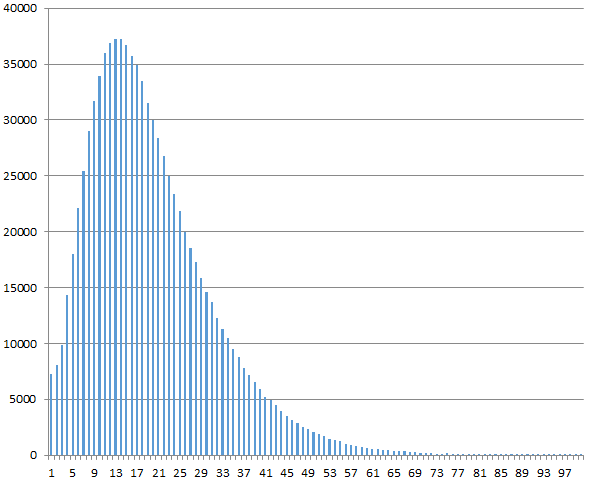
\includegraphics[width=\linewidth]{figures/user_addons_histogram1.png}
\caption{Distribution of number of addons per user}
\label{fig:user_addons_histogram}
\end{figure}
\fi

\begin{figure}[t]
\centering
\begin{small}
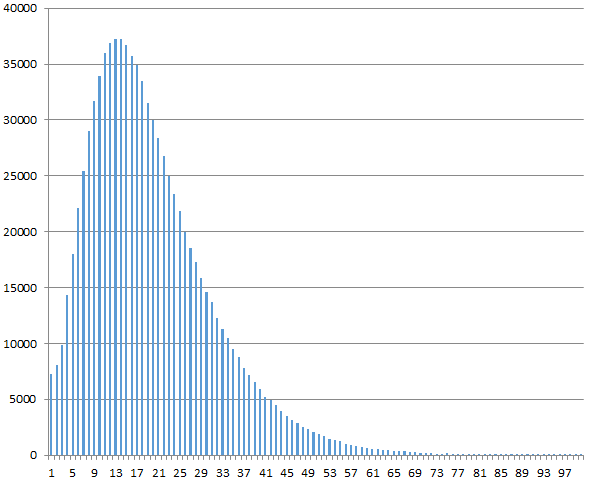
\includegraphics[scale=.8,angle=0]{figures/user_addons_histogram1.png}
\end{small}
\caption{Distribution of number of addons per user}
\label{fig:user_addons_histogram}
\end{figure}

\subsection{Data properties}

Our focus is on {\it users} and {\it addons}. While the database includes details about each user, such as his/her origin IP, ISP, and country, we do not make use of any personal information in this study. {\it Addon} instances are described as a set of attribute values extracted from the user's machine, as follows:
\begin{itemize}
\item Addon type--addon types form a closed set, where prevalent values are `extension', `toolbar', or `BHO' (an Internet Explorer addon).
\item File name--the full path at which the addon software is installed on the user's machine. 
\item Name--the addon's name. 
\item Description--a textual description field. 
\end{itemize}
Figures \ref{fig:db_addons_snapshot} and \ref{fig:db_addons_snapshot_desc} include example addon records associated with two different users. As shown, it is often the case that the addon's file path or description fields are not populated (addon descriptions are missing for the first user, and the path information is missing for the second user). We found that the types of information specified were often browser-dependent. For each user--addon pair, at least one attribute (path, name, or description) is present in the data.

\begin{figure}[t]
\centering
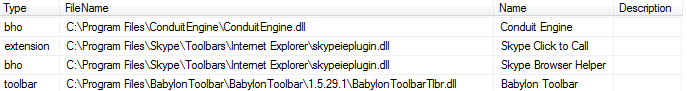
\includegraphics[angle=0]{figures/db_addons_snapshot.png}
\caption{User addons record: user A}
\label{fig:db_addons_snapshot}
\end{figure}

\begin{figure}[t]
\centering
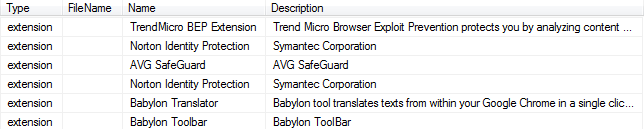
\includegraphics[angle=0]{figures/db_addons_snapshot_desc.png}
\caption{User addons record: user B}
\label{fig:db_addons_snapshot_desc}
\end{figure}

Importantly, similar addon software may be described by multiple different records, i.e., the addon records lack normalization. Figure \ref{fig:addons_versioning_snapshot} illustrates this variability across records, which we consider to be coreferent. Sources of variance include different installation paths, availability or absence of attribute values, and different software version numbers (e.g., 1.8.7.2 vs. 1.6.4.6 in Fig. \autoref{fig:addons_versioning_snapshot}). Furthermore, the user base is international and is therefore multilingual. 

\begin{figure}[t]
\centering
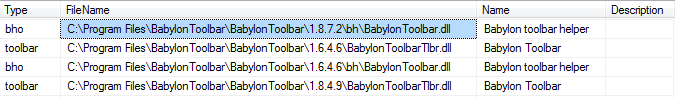
\includegraphics[angle=0]{figures/addons_versioning_snapshot.png}
\caption{Example of coreferent addon records, which differ on software version number}
\label{fig:addons_versioning_snapshot}
\end{figure}

Finally, we note that the database includes no tracking of user's or other programs' actions. It is therefore impossible to determine which party initiated the installation (or removal) of an addon; concretely, we cannot infer whether a particular addon has been installed (or removed) by the user or automatically, by a hostile or protecting program. 

\subsection{Graph representation}
\label{tab:graph_representation}

\iffalse
\begin{table}[t]
\begin{center}
\begin{small}
\begin{tabular}{llll}
\hline 
\textbf{source type} & \textbf{edge type} & \textbf{target type} \\
\hline
{\it user} & has-addon & {\it addon} \\
\hline
{\it addon} &  has-addon$^{-1}$ & {\it user} \\
{\it addon} & has-term & {\it term} \\
\hline
{\it term} & has-term$^{-1}$ & {\it addon} \\
\hline
\end{tabular}
\end{small}
\end{center}
\caption{\label{tab:graph_structure} The graph node and edge types}
\end{table}
\fi

We compactly represent our dataset using a relational graph schema. Each node in the graph represents a unique object that belongs to one of the following node types:
\begin{itemize}
\renewcommand{\labelitemi}{$\bullet$} 
\item {\it User}--an individual user is represented as a graph node that carries his/her unique user id. 
\item {\it Addon}--these nodes correspond to specific addons, defined as the concatenation of all of the addon's attributes, namely, file path, addon name and description.
\item {\it Term}--we break the text strings that comprise addon names into individual terms, and have distinct terms represented as graph nodes. As will be discussed below, we wish to connect {\it addon} nodes via their common {\it terms} in the graph.
\end{itemize}

\begin{figure}[!htbp]
\centering
\begin{small}
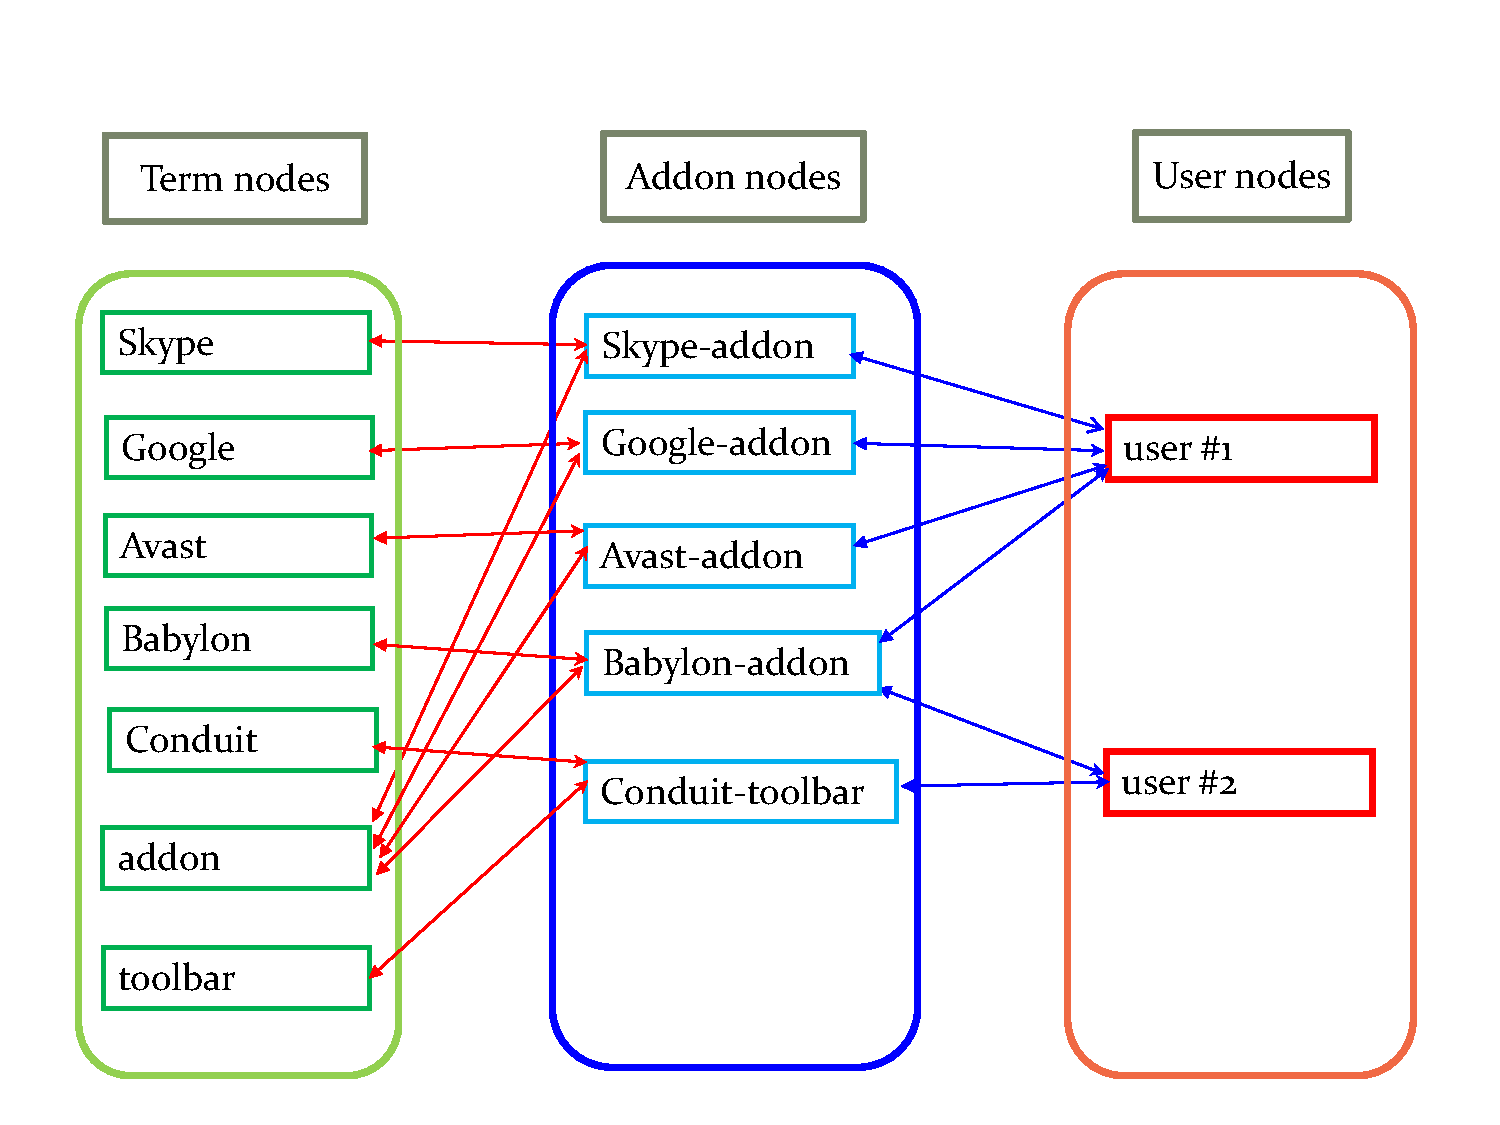
\includegraphics[width=0.75\textwidth]{figures/symbolic_graph.pdf}
\end{small}
\caption{User-Addons-Terms connections}
\label{fig:symbolic_graph}
\end{figure}

There are two types of edges in the graph. The first type of edges represents the structural association between each user and each {\it addon} installed on his/her machine PC. The second type of edges links each {\it addon} node to all {\it term} nodes that comprise its Bag-of-Terms representation. Inverse edges exist between every connected node pair so the graph may be viewed as undirected. 

Figure~\ref{fig:symbolic_graph} illustrates the graph structure. A user is represented as a graph node, which is connected to all its corresponding addon nodes with undirected edges. Each addon node, in turn, is connected to all its term nodes. In the specific example of Figure~\ref{fig:symbolic_graph}, {\it user 2} has two addons ({\it Babylon-addon} and {\it Conduit-toolbar}), which are connected to their term nodes ({\it Babylon}, {\it Conduit}, {\it addon} and {\it toolbar}).
To construct the graph, we iterate over all the users in our dataset and create user nodes. For each user, we iterate over all his/her addons, and map each addon string to a unique graph node. Finally, each {\it addon} node string is tokenized and lower-cased into single words, and each unique word is mapped to a respective {\it term} node. 

Besides being compact, the graph representation is advantageous in that similar entities reside in high proximity to each other. Consider, for example, two {\it addons} `Skype-US' and `Skype-UK', which have non-identical names, but share the term `Skype', which indicates in this case that they are variants of the same addon. Figure~\ref{fig:terms_layer} shows how terms nodes help to construct a connected graph where similar nodes are close to each other. Two disconnected segments on the left panel get connected to each other through the `Skype' term node, which leads to a close relatedness between {\it User 1} and {\it User 2}. In our experiments, we will apply random walks in the graph in order to assess similarity---or relatedness---across users, addons and terms.  

%\begin{figure}[!htbp]
\begin{figure}[t]
\centering
\begin{subfigure}[b]{0.49\textwidth}
	\centering
	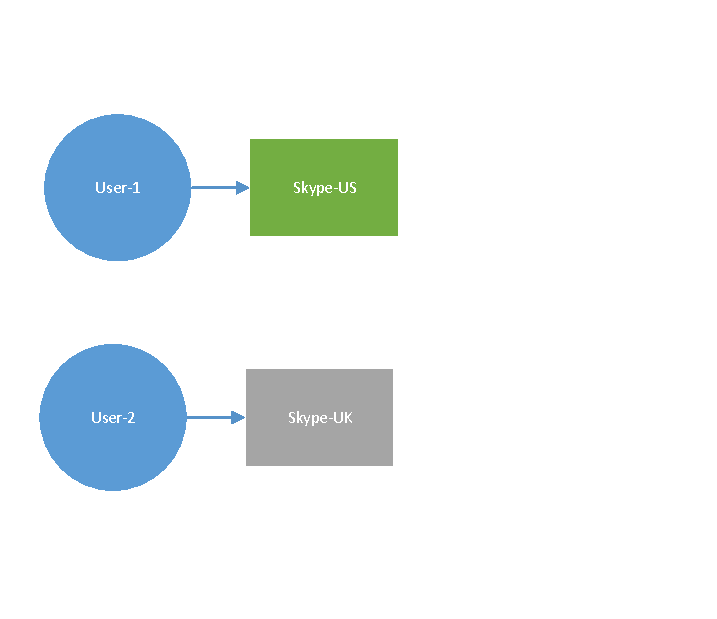
\includegraphics[width=\textwidth]{figures/skype_exampe1.pdf}
	\caption{Without terms layer}
%	\label{fig:skype-no-terms}
\end{subfigure}
\begin{subfigure}[b]{0.49\textwidth}
	\centering
	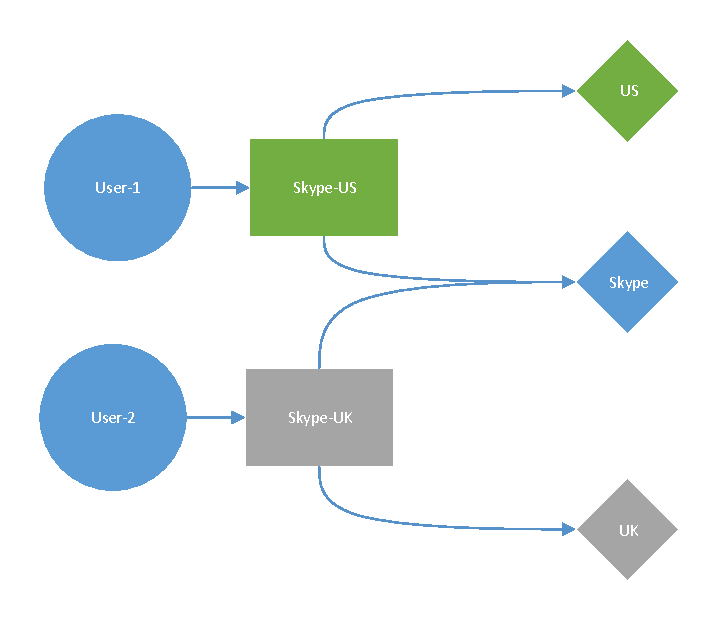
\includegraphics[width=\textwidth]{figures/skype_exampe2.pdf}
	\caption{With terms layer}
%	\label{fig:skype-with-terms}
\end{subfigure}
	\caption{Terms layer example}
	\label{fig:terms_layer}
\end{figure}


\subsection{Graph statistics}

The experimental dataset corresponds to a graph that consists of over 1.3 million nodes and over 18.5 million edges. Detailed statistics are provided in \autoref{tab:node_types}.

\begin{table}[H]
\centering
\begin{small}
\begin{tabular}{|l|r|}
\hline
\textbf{Type}                                                                & \textbf{Number of nodes} \\ \hline
all nodes                                                                    & 1,331,814         \\ \hline
user nodes                                                                   & 907,844          \\ \hline
addon nodes                                                                  & 256,458          \\ \hline
term nodes                                                                   & 167,512          \\ \hline
high degree nodes (\textgreater500)                                          & 2,430            \\ \hline
all edges                                                                    & 18,552,622        \\ \hline
user-addon edges                                                             & 17,612,159        \\ \hline
addon-term edges                                                             & 940,463          \\ \hline
\end{tabular}
\end{small}
\caption{Graph statistics}
\label{tab:node_types}
\end{table}

A property of many natural networks is that they exhibit a power-law degree distribution~\citep{albert1999internet}. \autoref{fig:zipf} depicts the node degree distribution for {\it addon}, {\it user} and {\it term} nodes on a log-log scale. As shown, addons in Figure~\ref{fig:zipf}(a) are distributed according to the Zipf's law, with a roughly linear curve. The term degree distribution curve shows a similar trend, while the user degree distribution curve is heavier on low-degree users (which is consistent with Figure~\ref{fig:user_addons_histogram}).

\begin{figure}[t]
\centering
\begin{subfigure}[b]{0.30\textwidth}
	\centering
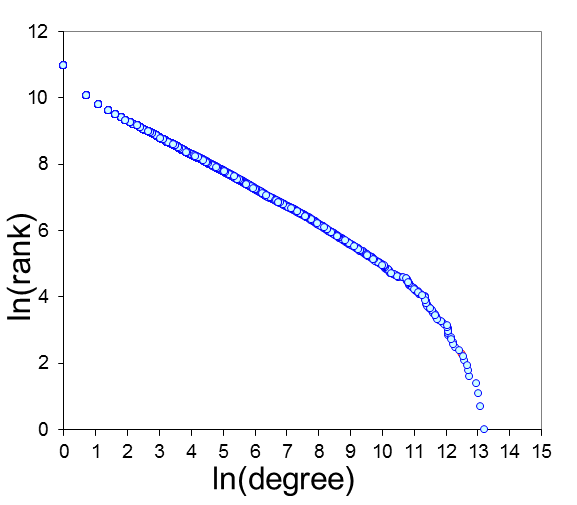
\includegraphics[scale=0.30]{figures/zipf_addon1.png} \\
\caption{addons} 
\label{fig:power_law_addons}
\end{subfigure}
\begin{subfigure}[b]{0.30\textwidth}
	\centering
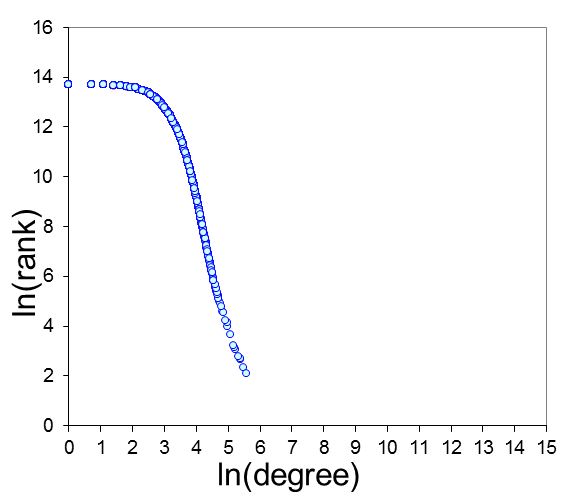
\includegraphics[scale=0.30]{figures/zipf-users1.png} \\
\caption{users} 
\label{fig:power_law_addons}
\end{subfigure}
\begin{subfigure}[b]{0.30\textwidth}
	\centering
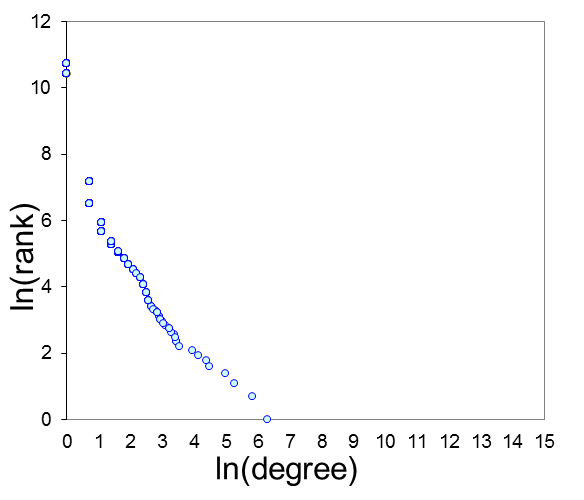
\includegraphics[scale=0.30]{figures/zipf-terms1.png} \\
\caption{terms}
\end{subfigure}
%	\centering
%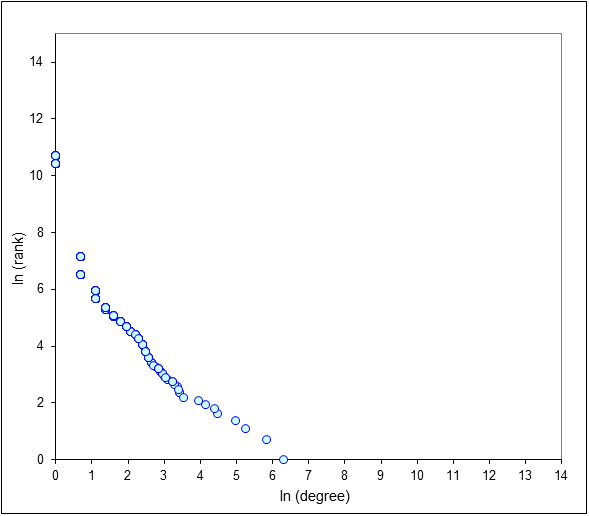
\includegraphics[scale=0.33]{figures/zipf-terms.png} \\
%(c) terms \\
\caption{Log-scale rank vs. degree plots of addons (a), users (b), and terms (c)}
	\label{fig:zipf}
\end{figure}

\section{The memory of a `missing' addon}
\label{chap:user_ecosystem}


Having described the local distributions of addons at users as a graph, we now wish to address the following question:

{\it Given only partial information about the population of addons residing at the machine of an individual user--can one infer the identity of additional species (addons) that exist in that environment?}

To the extent that it is possible to predict with high certainty member species of a given environment, this will indicate that addon populations exhibit {\it memory}, a basic property required for {\it ecological resilience}, thus supporting the claim that addons form a ecosystem. 

In this section, we first cast this question into a link prediction task and describe our approach for recovering the identity of missing addons using graph-based association metrics. We then report the results of an extensive set experiments proving that information about the environment is indeed helpful and necessary for recovering the identities of missing addons. 

\subsection{The prediction task}
\label{sec:task}

We evaluate the above-stated question empirically through link prediction experiments. In the experiments, a direct link between a random {\it user} and {\it addon} node pair is artificially removed, and the identity of the `missing' addon is then predicted based on information about remaining {\it addon} members at the user's environment. In this work, we apply the Personalized
PageRank (PPR) algorithm to rank the thousands of known {\it addons} by their graph-based association with the user's environment. 

More formally, let $U$ denote the set of users represented as nodes in the underlying graph $G$. Every individual user $u\in U$ is linked in $G$ to the set of addons installed on $u$'s machine, $A(u)$. Having disconnected the link between a random user $u_i$ and a single item $a_j \in A(u_i)$, we wish to evaluate the extent to which the missing link between $u_i \Rightedge a_j$ can be recovered based on the remaining information about the user's environment $A(u_i)'=A(u_i) \setminus \{a_j\}$ and $G$. Using information retrieval terminology, in what follows we will refer to $A(u_i)'$ as a {\it query}. Candidate responses in this case are all {\it addons}, which are not known to be associated with the user, i.e., $(A \setminus A(u_i)')$, having this candidate set include the target response $a_j$. These candidate nodes are ranked by to their estimated relevance to the query. Accordingly, performance is evaluated quantitatively with respect to the rank of the `missing' {\it addon} $a_j$ across multiple instantiated queries. 

\subsection{Approach}
\label{sec:method}

We employ Personalized PageRank (PPR) \citep{page1999pagerank} to compute query-specific relevance scores based on the link structure of the graph. A comprehensive overview of the PPR measure can be found elsewhere (cite). A brief summary of the algorithm follows for the reader's convenience.

The Personalized PageRank method follows the well-known PageRank algorithm, originally designed to assign a `centrality' score to Webpages. PageRank models the behavior of a random surfer, who at any given time, chooses to either follow a hyperlink to another Webpage, or to jump (`reset') to some random page on the Web. The probability distribution of finding the surfer at any of the graph nodes at time step $d$ is computed iteratively, as follows:
\begin{equation}
V_{d+1} = (1-\alpha) \left[{1 \over N}\right]_{1 \times N} + \alpha A^\top V_d
\label{eq:pagerank}
\end{equation}
where the total number of nodes (Webpages) is $N$, and $A^\top$
is a transition matrix, modeling the probability that the surfer move
to page $j$ from page $i$ following a hyperlink. The probability that
the surfer chooses to proceed by following some hyperlink is $\alpha$, and the probability of the alternative action, i.e., resetting the walk, is ($1-\alpha$) .
\iffalse
$A^\top$ distributes a node's probability uniformly among the pages it links
to, i.e.
\begin{equation}
A^\top_{ij} = \left}
\begin{array}{lll}
{1 \over |ch(i)|} & \mbox{if there is an edge from $i$ to $j$} \\ 0 &
\mbox{otherwise}
\end{array}
\right.
\label{pagerank_edge_weights}
\end{equation}
where $ch(i)$ is the set of nodes that have an outgoing link from $i$
(the children of $i$).
\fi 
The distribution $V_d$ is guaranteed to converge to a unique stationary distribution $V^*$, in which node scores designate the respective documents' centrality in the network. In general, a node is assigned a high PageRank score if the sum of the ranks of its backlinks is high, that is, if it is linked to by other important Webpages.

The PageRank centrality scores reflect the network's structure. The {\it Personalized PageRank} variant further biases the random walk model to
generate rankings that reflect personal user preferences. This bias is modeled by a natural adaptation of the random walk scheme---rather than having the surfer reset to any graph node uniformly at random, the reset operation is confined to a subset of graph nodes of interest. That is, the random walk scheme modified as follows:
\begin{equation}
V_{d+1} = (1-\alpha) V_u + \alpha A^\top V_d
\label{eq:ppr}
\end{equation}
where $V_u$, hereby the {\it query}, denotes a distribution over nodes that are of interest to user $u$. The Personalized PageRank scores, derived from the corresponding stationary state distribution, reflect structural similarity, or relevance, of graph nodes with respect to the query nodes.

It has been shown that the Personalized PageRank score for a target node $z$ and any single query node $x$ equals a summation over all the connecting paths between $x$ and $z$ (including cyclic paths, and paths that cross $z$ multiple times), where paths are weighted by their traversal probability \citep{jeh2003scaling,fogaras2004towards}. In other words, the graph walk distributes probability mass from the start distribution $V_u$ through edges in the graph---incidentally accumulating evidence of similarity over multiple connecting paths. Due to the reset operation, having a fixed fraction of probability mass reassigned to the query nodes at each time step, the weights of the paths between $x$ and $z$ are exponentially decayed as their length increases. This implies that graph nodes that can be reached from the query nodes over shorter connecting paths, as well as over multiple connecting paths, are considered more `important' with respect to the query. 

\subsubsection{Predicting the missing addon using PPR}

We address link prediction as a ranking problem, assessing the relevance of graph nodes that denote {\it addons} by their structural
similarity to the user's environment in the graph. Concretely, we set $V_u$ to be uniform over $A(u)'$ and zero otherwise. The constructed transition matrix $A^\top$ assumes equal importance to all of
the graph edges, that is, the transition probability from node $i$ to
a linked node $j$ is defined as: $(V_d)_{ij}={1 \over \mid N_i \mid}$,
where $N_i$ is the set of nodes linked over an outgoing edge from $i$. For example, suppose that node $i$ is linked to two {\it term} nodes and five {\it user} nodes; then, the probability of reaching any of these nodes using the transition operation equals ${1\over 7}$. It is generally possible to tune varying graph edge weights to denote their degree of importance, and to further learn a selective set of meaningful paths in the graph that link query with target nodes \citep{minkov2010improving,lao2010relational}. We leave the exploration of learned random walk measures to future work. 

The computed Personalized PageRank vector assigns a score to every node in the graph. Based on these scores, we generate a ranking of {\it addon} nodes. It is conjectured that the `missing addon' will be among the top-ranked items in the list, due to its high structural coherence with the set of addons that comprise the query. Specifically, we expect PPR similarity scores to flow from the query to candidate {\it addon} nodes over the following path types, reflecting several flavors of structural similarity:
\begin{itemize}
\item {\it User-based similarity}: Related addons may be connected to the query nodes over the short path  {\it addon} $\Rightarrow$ {\it user}
   $\Rightarrow$ {\it addon}. In words, this path type propagates probability scores from any query addon to other users who have the same addon installed on their machine. Walking away from these {\it users} to other {\it addons} attributes high weights to addons that frequently co-occur with the query addon in the same machines. \iffalse As the query consists of multiple {\it addon} nodes, the resultant PPR scores are expected to prioritize {\it addons} that co-exist on users' machines with multiple common addons.\fi   
\item {\it Term-based similarity}: As demonstrated in \autoref{tab:graph_representation}, the name and descriptions of addon instances exhibit lexical variation. For example, the names of addons may vary with respect to the software's version number. Coreference resolution can take place via the path {\it addon} $\Rightarrow$ {\it term} $\Rightarrow$ {\it addon}. That is, the graph-based similarity metric tends to connect {\it addons} pairs that have multiple {\it terms} in common. 
\end{itemize}
The stationary distribution of the random walk process manifests long-range relationships in the graph, consisting of various concatenations of the paths listed. We therefore expect that co-occurrence of coreferent {\it addons} will also be reflected in the random walk results.

\subsection{Experimental setup}

\subsubsection{Query generation}

We derive labeled queries from our corpus for evaluation purposes.  Each query corresponds to a randomly selected user $u$. Having selected the user node $u$, we further randomly select one of its linked {\it addons} $a$. The selected addon is then eliminated artificially from the user's `profile', i.e., the link between the nodes denoting $u$ and $a$ is removed from the graph. The process of generating an individual labeled example is outlined in Figure \ref{fig:example-gen}. In the experiments, we evaluate the extent to which the link to the missing addon can be recovered. As a query, we take the rest of user $u$'s addons. We then run PPR on the entire graph, with respect to the constructed query. 

\begin{figure}
\begin{enumerate}[(a)]
\begin{small}
\item Pick uniformly at random a {\it user} node $u$ from the graph.
\item Find the set of all {\it addon} nodes linked to $u$, $A_u$.
\item Pick uniformly at random an addon node $a$ from the set $A_u$. 
\item Remove the edge between nodes $a$ and $u$ in the
  graph. 
\item Let the query $V_u$ be a uniform distribution over $A_u \setminus \{a\}$,
  and the correct response to the query (the `label') be $a$. 
\end{small}
\end{enumerate}
\caption{The process of generating an individual labeled example}
\label{fig:example-gen}
\end{figure}

\subsubsection{Evaluation measures}

Having produced a ranked list of addons per query, we assess performance using metrics adapted to the evaluation of ranked lists. Note that in our settings, there is a single known `correct' answer, i.e.~the missing addon. The evaluation metrics assess the extent to which the correct answer is included at the top of the ranked list of addons, across the set of test queries. Obviously, user and term nodes, as well as the query addon nodes, are discarded from the evaluated ranked list. A short description of the evaluation measures follows.

\paragraph{Recall at rank $k$}
This is the fraction of queries, in which the relevant response is included among the top $k$ ranks (see also \cite{minkov2010improving}). Concretely, the non-interpolated recall at rank $k$ of a given ranked list is defined to be 0 for each rank $k = 0, \dots, k_{i-1}$, where $k_i$ is the rank that holds the single correct entry, and 1 for ranks $k\geq k_i$. The (mean) recall at rank $k$ averages the recall scores at each rank $k$ across the rankings of multiple queries. Thus, mean recall is in the range [0,1] at each rank $k$. For example, if recall at rank 3 is 0.7, this means that for 70\% of the queries, the correct answer appears among the top 3 ranks of the generated ranked lists.

\paragraph{Mean Reciprocal Rank (MRR)}

The mean reciprocal rank metric \citep{voorhees1999trec} considers the position of the first correct answer in the ranked list.  As formalized in Eq.~\eqref{eq:mrr}, the non-interpolated reciprocal rank is the inverse of the position of the correct item (addon) in the ranked list for a given query. The MRR score is the mean reciprocal rank across all of the queries. Unlike the recall-at-rank measure, which ignores the results below rank $k$ for evaluation purposes, MRR is based on the full list of ranked items. 
\begin{equation}
 MRR = \frac{1}{Q} \displaystyle\sum\limits_{q=1}^{Q} \frac{1}{rank_q}
\label{eq:mrr}
\end{equation}

In order for the evaluation to be sound, we apply the above metrics to evaluate query sets that consist of $1000$ labeled examples of randomly sampled user-addon pairs per experiment. Furthermore, in order to guarantee the soundness of the evaluation, each experiment was repeated using four sets of queries (4$\times$1000). We report the average of the evaluation scores (4 in total) per query set, alongside their standard deviation.  

\subsubsection{Implementation details}

In all of our experiments, we make use of a fast and memory-efficient implementation of Personalized PageRank included in {\it igraph} \citep{igraph}, a software library optimized for the processing large-scale graphs. We ran the experiment using a standard PC machine using the 64-bit version of igraph. The computation of PPR scores was highly efficient, as the whole graph is loaded into memory. A batch of 1000 PPR runs completed within a few hours.

The rankings generated using PPR may be affected by design choices concerning the graph structure and the random walk scheme. In the experiments, we set the teleport probability parameter $\alpha=0.85$ following previous works \citep{boldi2005totalrank}. In general, due to the exponential decay over distance from the query nodes implied by PPR's random walk formula, the teleport probability value has a negligible effect on the produced rankings.

\subsubsection{Tuning the graph design}

Addon names often include full file-system path information, e.g.,
`C:/Program Files (x86)/Skype/skype1.dll'. In our experiments, we remove path prefixes 
(such as `C://Program Files (x86)/skype') from addon names. The reason is that we wish to represent every unique addon as a distinct node in the graph, while including path details in the addon name result in multiple copies of the same addon---solely due to minor discrepancies in the installation process. 

As discusses earlier, we include {\it terms} in the graph, in order to model term-based lexical similarity between coreferent (or generally similar) addon descriptions. Ideally, similar addons with slight name differences, e.g., different version numbers, should be unified as part of the random walk. Splitting the addon names into tokens and linking the respective {\it addon} and {\it term} nodes should maintain connectivity between multiple version of the same {\it addon}, where consequently this should improve the graph relatedness measure. On the other hand, linking {\it addons} over shared {\it terms} may lead to an undesired outcome. For example, suppose that an {\it addon} that has to do with video streaming has the term `video' as part of its name; other {\it addons} reached by traversing a term-hopping path may have similar functionality, but be competing rather than ally addon software. Our experimental results having removed the {\it term} nodes from the graph showed that overall, term modeling has positive albeit modest impact on the produced rankings. We found that {\it addon} nodes are typically connected to a large number (hundreds) of {\it user} nodes, but only to a very few {\it term} nodes. Since the random walk distributes probability mass uniformly over all neighbors of a source node, the total probability flow through the {\it term} nodes is relatively small. Assigning higher weight to links leading to {\it term} nodes (see~\cite{minkov2010improving}) will increase their traversal probability and increase their impact. We leave the exploration of this possibility for future work.

\subsection{Results: evaluating the effect of ecological memory}
\label{sec:user_main_results}

In order to assess the extent to which information about the remaining addons in a user's machine is helpful for predicting the identity of a `missing' addon, we compare the prediction results using PPR with two non-personalized alternative ranking methods: ranking {\it addons} by `popularity', as well by their (non-personalized) PageRank scores. It is customary to use random ranking as a baseline as well. However, since we rank hundreds of thousands of addons, random ranking is supposed to produce extremely poor results, so we do not report them.

\paragraph{Popularity baseline} 

To predict the `missing' addon, one may rank the known {\it addon} items by their popularity, determined by the total number of users associated with each addon in the corpus. According to this non-personalized approach, all users are presented with the same addon popularity list. Despite its simplicity, the popularity algorithm demonstrates strong results when item popularity distribution follows the power law. 

\paragraph{PageRank baseline} 

For each addon, we compute its non-personalized PageRank score in the underlying graph. The PageRank scores reflect the structural centrality of {\it addon} nodes in the graph. We are interested in comparing PPR performance with this non-personalized variant of the random walk algorithm.

Figure~\ref{fig:main} shows recall-at-$k$ results using PPR, as compared against ranking-by-popularity and by PageRank scores. Full results, including the mean and standard error of MRR performance are presented in Table~\ref{tab:full}. As can be seen in Figure~\ref{fig:main}(a), PPR rankings yield consistently superior performance to the non-personalized baseline methods. Recall-at-rank-10 using PPR is as high as 0.354, further extending towards recall of 0.660 and 0.801 at the top 50 and 100 ranks, respectively. Compared with popularity-based ranking, recall-at-10 performance improves at an impressive rate of 45.7\% using PPR (0.354 vs. 0.243). Improvement rates at rank-50 and rank-100 are 18.9\% and 12.7\%, respectively. These results indicate that addons form tight bonds in the Web browser ecosystem. 

Interestingly, performance using the popularity- and PageRank-based rankings is nearly identical. This result is not very surprising as the most popular {\it addons} are likely to be prominent in terms of graph centrality.

\begin{figure}[!htbp]
\centering
\begin{subfigure}[b]{0.49\textwidth}
	\centering
	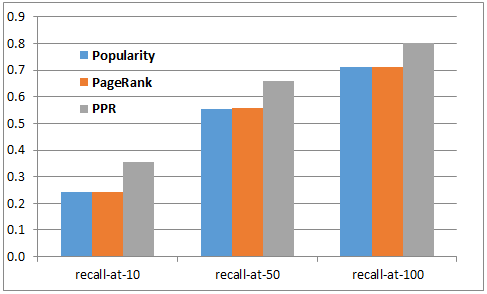
\includegraphics[width=\textwidth]{figures/pop-final.png}\\
	(a)
%	\caption{Without terms layer}
%	\label{fig:skype-no-terms}
\end{subfigure}
\begin{subfigure}[b]{0.49\textwidth}
	\centering
	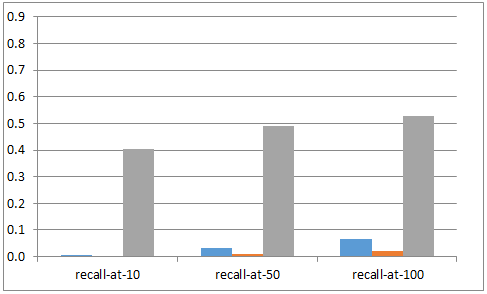
\includegraphics[width=\textwidth]{figures/sans-popular-final.png}\\
	(b)
%	\caption{With terms layer}
%	\label{fig:skype-with-terms}
\end{subfigure}
	\caption{Main results: recall at top ranks for the full graph (a), and the graph excluding the most popular addons (b)}
	\label{fig:main}
\end{figure}


\begin{table}[!htbp]
\small
\centering
\caption{Recall and MRR results, averaged over 4 independent runs (standard error of the mean is shown in the brackets)}
\label{tab:full}
\begin{tabular}{llcccc} \hline
	& & Recall-at-10 & Recall-at-50 & Recall-at-100 & MRR	 \\
\hline
\multicolumn{6}{c}{FULL GRAPH} \\
\hline
& POP & 0.243 (0.007) & 0.555 (0.017) & 0.711 (0.012) & 0.104 (0.004) \\
& PR & 	0.243 (0.007) & 0.559 (0.016) & 0.711 (0.012) & 0.104 (0.004) \\
& PPR	& \textbf{0.354}	(0.011) & 0.660	(0.009) & 0.801 (0.004) & \textbf{0.151}	(0.006) \\
\hline
No terms & POP & 0.240 (0.009) & 0.553 (0.012) & 0.719 (0.007) & 0.101 (0.005) \\
& PR & 0.240 (0.009) & 0.563 (0.014) & 0.719 (0.007) & 0.101 (0.005) \\
& PPR	& 0.350	(0.014) & \textbf{0.665}	(0.008) & \textbf{0.809}	(0.014) & 0.146	(0.008) \\
\hline
%Full path & POP & 0.065 (0.005) & 0.177 (0.010) & 0.224 (0.010) & 0.023 (0.004) \\
%& PR & 0.185 (0.013) & 0.409 (0.016) & 0.538 (0.012) & 0.079 (0.010) \\
%& PPR	& 0.294	(0.017) & 0.592	(0.015) & 0.708	(0.010) & 0.150	(0.008) \\
\hline
\multicolumn{6}{c}{WITHOUT POPULAR NODES} \\
\hline
 & POP & 	0.006 (0.004) & 0.034 (0.009) & 0.065 (0.009) & 0.004 (0.001) \\
 & PR	& 0.001	(0.000) & 0.009	(0.009) & 0.022	(0.003) & 0.001	(0.000) \\
& PPR	& 0.405	(0.007) & 0.491 (0.007) & 0.527	(0.004) & 0.320	(0.005) \\
\hline
No terms & POP & 	0.000 (0.000) & 0.000 (0.000) & 0.000 (0.000) & 0.000 (0.000) \\
& PR & 	0.001 (0.002) & 0.012 (0.007) & 0.027 (0.002) & 0.001 (0.000) \\
& PPR & 	0.401 (0.027) & 0.483 (0.027) & 0.521 (0.022) & 0.322 (0.027) \\
\hline
%Full path & POP & 	0.004 (0.003) & 0.019 (0.006) & 0.033 (0.007) & 0.003 (0.001) \\
%& PR & 	0.032 (0.010) & 0.033 (0.010) & 0.034 (0.010) & 0.001 (0.000) \\
%& PPR	& \textbf{0.496}	(0.017) & \textbf{0.575}	(0.022) & \textbf{0.602}	(0.016) & \textbf{0.415}	(0.020) \\
\hline
\end{tabular}
\end{table}

Table~\ref{tab:full} and Figure~\ref{fig:main}(b) include the results of a similar experiments over a graph variant, in which high-degree nodes were removed. Previous studies have shown that PageRank exhibits some bias in favor of high-degree nodes~\citep{tong2006center,budalakoti2012}. Others showed that the removal of high-degree nodes from an undirected power-law graph leads to a small approximation error, while improving the computational cost of the random walk~\cite{sarkar2010tractable}. We therefore experimented with pruning high-degree nodes, for which the out-degree is equal or greater than 500. As shown in Figure~\ref{fig:zipf}, only a small fraction of the most popular {\it addons} are pruned in this way. Importantly, given a graph variant in which these `popular' nodes are removed, the missing addons (randomly sampled from the reduced graph) are now limited to lower-frequency addons, which are more challenging to predict. 

As shown in Figure~\ref{fig:main}(b) and Table~\ref{tab:full}, performance of the popularity-based approach plummets when popular addons are removed from the graph: recall-at-10 is nearly zero (0.006) and recall-at-100 is also very low (0.065). Non-personalized PageRank's results are even lower. In contrast, PPR remains effective: recall-at-rank-10 is 0.405 using PPR, reaching 0.491 and 0.527 at ranks 50 and 100, respectively. While recovering links to non-popular addons may be more challenging, recall-at-10 is in fact higher using PPR in this scenario (0.405 vs.~0.354). This indicates that popular nodes, which tend to occupy the top ranks, indeed `push' relevant yet less popular nodes to lower positions in the ranked lists.  

Our conclusion from these experiments is that there exists strong structural association between the addons installed on a user's machine, to the extent that it is possible to recover the identity of an addon if removed from the environment with high success: indeed, there is a 40.5\% chance to see the missing addon among the top 10 addons in the ranked list of over 250,000 addons! The Web browser ecosystem is resilient in this respect, supporting the analogy to biological ecosystems.

\subsection{Discussion}

In this section, we evaluated the coherence among the community of addons installed on a user's machine. We found that Personalized PageRank performs well on the task of identifying a missing addon given information about its environment. Alternative one-fits-all rankings of addons (based popularity or graph centrality) yielded substantially inferior results, indicating that addon populations are strongly interconnected.  

Multiple factors may underlie this phenomenon. The population of addons on a user's machine is clearly affected by the user's personal preferences, regardless of the extent at which the user is actively involved in maintaining his/her Web browsing environment. Another factor is functionality: some addons are complimentary to each other. Important, and of high interest, is addon binding as a result of interventions of addon manufacturing companies in the addon installation process. Coexistence of addons of different companies may be an indication of business alliances. In contrast, rivalry between addon distributors may be reflected in exclusiveness of their addons. 

\section{PPR-based analysis of addon coexistence}
\label{chap:Symbiosis}

Here we investigate the addon coexistence phenomenon. We observe that existence of some addons on a user's machine tends to be affected by other addons, i.e. when addons of one company are installed, addons of another company have greater or lower chances to be installed on the same machine. The positive effect of coexistence will hereafter be referred to as \emph{symbiosis}, while the negative effect as \emph{clash}.

The symbiosis phenomenon often occurs when addons of some companies are distributed via third parties: an addon's installation is offered to a user as a part of some other product installation process, for example, while the user installs Skype, the installation process suggests also installing Skype's `Click to Call' addon in all browsers. Another example is Ask Toolbar: at the time the data for this section was collected, Ask Toolbar installation was integrated with Java installation\footnote{\url{https://java.com/en/download/faq/ask_toolbar.xml}}. During the installation of Java, users were prompted to download and install the Ask Toolbar.

The clash effect can be observed when addons of one company get removed if addons of another company are installed on this machine or if the addons are not installed at all when another company's addons are pre-installed on the machine. For example, \emph{Kaspersky AntiVirus}, which develops addons for all browsers, treats \emph{iMesh} addons as threats and removes them from the computer\footnote{\url{http://securelist.social-kaspersky.com/en/kadvisories/KLA10420}}.

Needless to say, the life cycle of the addon ecosystem is mostly obscure for an outside observer. While some symbiotic effects may be visible to the users (e.g., an addon is prompted to be installed during an installation processes of another addon or a software product), some other symbiotic effects are hidden (e.g., those following undisclosed agreements between addon distributors). Clash effects, on the other hand, are almost always invisible. Besides a few well known conflicts between competing addon distributors that were widely covered in mass media\footnote{\url{http://goo.gl/AdlzUM}}, the competition is kept away from the eyes of general public. In this section, we disclose some of these effects and shed light on the macro-level addon ecosystem. 

The ability to detect a symbiosis or clash between addon distributing companies could turn handy for addon manufacturers. Information about symbiosis between two companies can help a third company to better analyze the powers and driving forces of the addon market, and to get better prepared for a potential competition. While it is unlikely that a company might not be aware of a symbiosis between its own addons and addons of another company, information about a clash that involves the company's addons may sometimes come unexpected. A typical addon manufacturer can benefit from the information about a clash between their own and someone else's addons in four ways:
\begin{enumerate}
\item Such a clash may imply that the user prefers someone else's addon over their own addon, so there might be a way to perform a comparative analysis of the two addons and learn how to improve their value proposition.
\item The clash could mean that a newly installed addon is hostile to other addons in an illegal way, i.e. it is the addon---and not the user---that uninstalls or sabotages another addon. Then, the distributor of the removed addon could report an abuse to the webstore owner.
\item An addon manufacturer can ask a third-party distributing company not to install an addon on a machine that keeps the hostile addon. Since in most cases, addon developers are paying distributors per install, this could decrease the developers' costs and rise their profits in a long run.
\item A clash can occur between addons of seemingly non-competing companies. This may happen when something goes wrong in the distribution process and the problem slips off the company's radar. The addon ecosystem is complex enough to make the distribution monitoring barely possible. If an unintended clash gets detected, the owner of the affected addon can contact the owner of the hostile addon and ask them to act.
\end{enumerate}

We chose nineteen companies (see~\autoref{table:companies_list}) among well-known addon distributors. These are companies that are most ``famous'' among the distributors of addons and toolbars. Interestingly, seven of the nineteen companies are antivirus and anti-malware companies. 
Although antivirus and anti-malware software aim to prevent unintentional addon installation, some antivirus companies are not only fighting unintentional addon installations but also distributing their own addons and toolbars. For example, AVG Anti Virus company distributes the AVG Security Toolbar which is detected by Avast Anti Virus as malware.  

In 2013, Avast Anti Virus published a list of top ten companies that were distributing their addons via third-party software installations\footnote{\url{https://blog.avast.com/2013/03/20/avast-browser-cleanup-at-work/}}---these addons were subject to removal. Surprisingly, the list published by Avast in 2015 did not change dramatically since 2013---many of these companies are in our list as well~(\autoref{table:companies_list}). Back in 2013, Avast identified over 3.3 million different browser extensions for the three major browsers. They also noticed that ``a lot of toolbars are available in different variants. These variations affect mostly the name''. 

In a blog post of July the 9th 2015, Avast describes the addon ecosystem of a user's Web browser. They highlight one of the major characteristics of the ecosystem: ``the addons fight against each other''\footnote{\url{https://blog.avast.com/2015/07/09/top-10-most-annoying-browser-toolbars/}}.
Based on Avast statistics on the forced removals of competing toolbars, some companies from our list are among the top ten offenders. For example, Conduit performed more than 13 million removals of their competitors' toolbars, ASK removed 11 million toolbars---and other companies were not far behind. Not surprisingly, Avast itself uses the same practice. A Techdows blog post\footnote{\url{http://techdows.com/2012/11/avast-comes-bundled-with-google-toolbar.html}} mentions that ``Avast is contradicting itself. Their latest product offers a built-in feature to rid your browser of toolbars, while offering a toolbar when installing their software.''

\begin{table}[!htbp]
\small
\centering
\caption{Companies list}
\label{table:companies_list}
\begin{tabular}{@{}lll@{}}
\toprule
{\bf Company name} & {\bf Example Product}               & {\bf Description}               \\ \midrule
ASK                & Ask Toolbar                 & Advertisement/Search company    \\
AVG                & AVG Safe Search addon       & AntiVirus/Advertisement company \\
Avira              & Avira Browser Safety        & AntiVirus company               \\
Babylon            & Babylon Toolbar             & Advertisement/Search company    \\
Blekko             & Blekko Toolbar              & Advertisement/Search company    \\
Conduit            & Conduit Toolbar             & Toolbar provider company        \\
Google             & Google Toolbar              & Advertisement/Search company    \\
Hotspot Shield     & Hotspot Shield VPN          & Security company                \\
iMesh              & iMesh Search                & Advertisement/Search company    \\
Incredimail        & MyStart by Incredimail      & Advertisement company           \\
Kaspersky          & Kaspersky Protection Plugin & AntiVirus company               \\
Montiera           & Montiera Toolbar            & Toolbar provider company        \\
Norton             & Norton Toolbar              & AntiVirus company               \\
Softonic           & Softonic Web Search         & Advertisement company           \\
SpeedBit           & Video Accelerator           & Software company                \\
SweetIM            & SweetIM Toolbar             & Advertisement/Search company    \\
Trend Micro        & Trend Micro Toolbar         & AntiVirus company               \\
Zone Alarm         & Zone Alarm Toolbar          & AntiVirus company               \\ 
Zugo               & Search Toolbar              & Advertisement company           \\ \bottomrule
\end{tabular}
\end{table}


\subsection{Experimental design}
\label{sec:experiment_des}

Since we analyze coexistence of \emph{addon manufacturing companies}, we first need to reveal which addon belongs to which company. An addon company most often distributes many addons---hundreds or even thousands. For example, \emph{Kaspersky URL Advisor Firefox addon} and \emph{Kaspersky Protection Chrome extension} are developed by the same company, so we say that they belong to the same species. Often, the same addon has different names---it is not easy to infer that addons with different names are in fact the same addon. We do not aim to infer that, instead, we are concerned with mapping addon names to company names. 

As discussed in Section~\ref{sec:datasets}, an addon is represented in our system by three attributes: name, full file-system path, and textual description. Any one (or any two but not all three) of the attributes may be empty. To infer which addon belongs to which company, we first apply a simple heuristic of detecting the company name within the three attributes of an addon. The rationale behind this is that the default path of an addon package installation often contains the company's name. If a user does not change the default option, the company name will most probably be included in the addon's path. The name and the description fields may contain the company name as well, see \autoref{table:addon_desc} for an example.

\begin{table}[!htbp]
\small
\centering
\caption{An example of a company's name contained in an addon's path or description}
\label{table:addon_desc}
\begin{tabular}{@{}|l|l|@{}}
\toprule
Path & C:\textbackslash{Program Files (x86)}\textbackslash{Kaspersky Lab}\textbackslash{Kaspersky Internet Security 2012}\textbackslash{avp.dll} \\ \midrule
Description & Kaspersky Protection extension \\ \bottomrule
\end{tabular}
\end{table}

After applying the company name search heuristic, we realized that representations of many addons that belong to companies from our list~\autoref{table:companies_list} do not in fact contain the company name. For example, an addon $tbbaby.dll$ does not contain any company name in any of its attributes, but does belong to Babylon\footnote{\url{http://www.shouldiremoveit.com/Babylon-English-Toolbar-31094-program.aspx}}.

In ~\autoref{chap:user_ecosystem}, we applied a Personalized PageRank (PPR) based algorithm for identifying a missing addon in a browser of a specific user. We proposed a method that took the entire set of the user's addons as a query input to PPR and produced the output of a ranked list of all addons in the system. We hypothesized that the missing addon would end up among the top addons in the ranked list. Our hypothesis was proved correct.

We apply a similar technique here, for mapping addons to their manufacturer companies. 
Just as in~\autoref{chap:user_ecosystem}, here we apply PPR to a graph with user, addon, and term nodes. We do not remove the high-degree addon nodes, however we do remove the addon file-system paths\footnote{Addon paths are instrumental for mapping addons to companies using the simple heuristic described above, however, for the PPR purposes, addon paths turn out to be too noisy to deal with.}. We never change the graph setting over the course of this section.

As a query for the PPR algorithm, instead of the set of addons existing in a user's browser, we now provide a set of addons that are known to belong to a company. We hypothesise that an addon that belongs to that company, and is not in the query, would ``pop-up'' in the ranked list. By ``popping-up'' we mean that the addon would be ranked closer to the top of the list, relatively to its original rank in the (non-personalized) PageRank. First, we run the non-personalized PageRank on the entire graph, and use the rank of each addon as the baseline position. For each company, we then run PPR and identify addons that substantially improve their position in the ranked list. For example, if an addon was at a rank of 15 in the non-personalized PageRank and moved to the rank of 14 in the PPR, we do not take it into account as its rank did not dramatically change. In contrast, if an addon was at a rank of 100 in the non-personalized PageRank and moved to the rank of 10 in the PPR, we consider it as a candidate to manual examination. For each addon that ``popped-up'' in the ranked list of a specific company's PPR, we manually validate that the addon actually belongs to the company.

We perform the procedure described above iteratively: after we discover addons that belong to a company, we add them to the query and rerun the PPR with the extended query. We stop the process once there are no more addons that dramatically change its rank. It turns out that two iterations are enough for the process to converge. Using this process, we discover 24 addons that ``popped up'' in the PPR ranked lists of companies from~\autoref{table:companies_list}. In a manual check of these 24 addons, we see 100\% precision: there was not one single addon that did not belong to the company in the query. An example of an addon that drastically changed its rank is the addon named \emph{tbmyba.dll}, which jumped from the 1200 rank position to the 15 rank position after running PPR with Babylon addons in the query. Indeed, we found out that this addon belongs to Babylon\footnote{\url{http://www.file.net/process/tbmyba.dll.html}}.

The success of this process reveals an interesting phenomenon: it turns out that there is a ``community'' of addons of the same company, and this community can be discovered via the Personalized PageRank weight propagation that starts with already known community members. One possible explanation for this phenomenon would be that it is a common practice for a company to offer a few of its addons for installation at the same time. For example, while Babylon is installing its Internet Explorer addon, it might also install its Chrome extension. Even if we manage to map the Internet Explorer addon to Babylon using the simple name matching procedure, the Chrome extension might not contain any attribute that would qualify it as related to Babylon. Still, our algorithm would discover it in a similar way it discovered a missing addon for a specific user. 
Another explanation may come from the \emph{collaborative filtering} theory~\citep{sarwar2001item}: users who have many addons in common might also have different addons of the same company---such addons will therefore be located in a close proximity of each other in the PageRank graph.

Now that we linked addons with their species (that is, their manufacturer companies), we are ready to analyze relations between the addon companies in the browser ecosystem. 
For each company from our list, we construct the PPR query to contain all the company's addons. The PPR output is the ranked list of all addons in the graph. Our goal is to find out addons of which companies ``pop up'' in the PPR as compared to non-personalized PageRank. If we identify a company whose addons are universally improving their rank in the PPR of another company, we may conclude that the two companies are engaged in a partnership. Using the ecological language, they are in \emph{symbiosis}. We also expect addons of a company to ``drop down'' the PPR ranked list, with respect to their position in non-personalized PageRank. If many addons of one company drop down in the PPR of another company, we conclude that the two companies \emph{clash} with each other.

\subsection{Symbiotic Relationships}
\label{sec:symb_relations}

\subsubsection{Addon Co-occurrence}
\label{subsub:co_occurrence}

Generally speaking, there may be multiple ways to detect symbiosis between addon manufacturing companies. One could suggest a simple way for detecting a symbiotic relationship which would be based on computing co-occurrence frequencies of addons on users' machines. If many addons of company $c_i$ are installed on the same machines where addons of company $c_j$ are installed, we may conclude that the two companies live in symbiosis with each other. To validate this hypothesis, we set up a simple experiment. For each pair of companies from our list (\autoref{table:companies_list}), we computed Jaccard index~\citep{jaccard1912distribution} which is the measure of overlap of two sets. We denote $\mathbf{M}_i$ the set of machines on which addons of company $c_i$ are installed. Analogously, we denote $\mathbf{M}_j$ the set of machines on which addons of company $c_j$ are installed. Jaccard index is then defined as:
$$
Jaccard(c_i, c_j) = \frac{|\mathbf{M}_i \cap \mathbf{M}_j|}{|\mathbf{M}_i| + |\mathbf{M}_j| - |\mathbf{M}_i \cap \mathbf{M}_j|},
$$
where the absolute value symbol means the cardinality of a set.

\begin{figure}[!htbp]
\centering
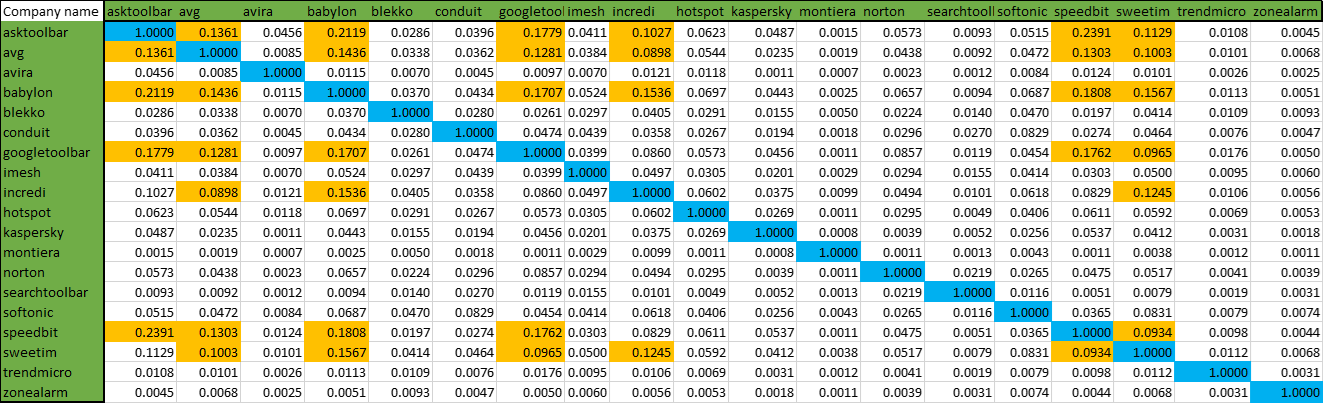
\includegraphics[width=\linewidth]{figures/JaccardMatrix.png}
\caption{All companies Jaccard index}
\label{fig:jaccard_matrix}
\end{figure}

The full matrix of Jaccard indexes is presented in~\autoref{fig:jaccard_matrix}. As we can see, some pairs of addon manufacturing companies have quite a significant co-occurrence: among all machines that keep addons of either company, up to 24\% machines keep addons of both companies. 

Somewhat counter-intuitively, the most significant co-occurrences do not appear corresponding to known collaborations between addon distributors. Even more counter-intuitively, some significant co-occurrences correspond to known competitions between addon distributors. An example is ASK, AVG, Google, and Babylon, all of which heavily co-occurring in our dataset. The four companies are distributing their own toolbars, thus competing with each other \footnote{\url{http://www.thewindowsclub.com/uninstall-babylon-yahoo-google-bing-toolbar}}. Moreover, some companies such as IncrediMail and Conduit, which are known for a cooperation with each other\footnote{Conduit eventually acquired IncrediMail, see~\url{http://goo.gl/4dybI6}.}, do not co-occur heavily.\footnote{These observations are correct for 2013 when our data was collected. Since then, the addon ecosystem has undergone many changes, e.g. Babylon shut down and Google stopped distributing its own toolbar. Still, most of the other players in the domain exist and there are some other new companies as well, see \url{https://blog.avast.com/2015/07/09/top-10-most-annoying-browser-toolbars/}}.

A possible explanation for the heavy co-occurrence of competing toolbars is actually in the intensity of the competition: major toolbar manufacturers are all working hard on ``sneaking in'' as many machines as possible. They all have very strong distribution mechanisms that cause a constant increase in their market penetration. While their toolbars get installed on many machines, they do not necessarily ``kick out'' toolbars of their competitors. Moreover, a direct clash is pretty rare because of enormous resources it would require given the size and significance of competing companies, as well as potential legal implications. Therefore, multiple toolbars get installed on the same machine, which is mostly the function of the user's tolerance: some users do not care / are not aware of / do not know how to prevent multiple toolbar installations. This leads to high co-occurrence of toolbars on some machines, but does not in the end indicate any collaboration between the toolbar distributors.

To summarize, addon co-occurrence computation does not appear to be the correct way to reveal symbiotic relationships between addon distributors.

\subsubsection{Personalized PageRank}

Following~\autoref{chap:user_ecosystem} and~\autoref{sec:experiment_des}, we use Personalized PageRank as the main mechanism to detect company symbiosis in the Web browser ecosystem. Addon ranking obtained by the standard (non-personalized) PageRank corresponds to the unbiased and undisturbed addon ecosystem in which every addon bears its relative importance value with respect to the others. Once the Personalized PageRank is applied, the ecosystem is disturbed with an artificial preference towards some of its elements. The artificial disturbance causes the entire ecosystem to adjust to the new condition, and such an adjustment reveals characteristics of the ecosystem that would not be visible in its original, undisturbed state. 

When all addons of a particular company comprise the PPR query, it is natural to expect the company's addons popping up in the ranked list. Other addons that are closely related to the addons of the query company might then follow the company's addons on their way to the top of the ranked list. The beauty of Personalized PageRank is in the fact that the essence of the relationship between the addons does not have to be disclosed a priori, nor explicitly modeled. This implies that hidden, invisible relationships between addon manufacturers can be discovered in the process.

Our research hypothesis is that addons that pop up in the PPR ranked list belong to a company $c_i$ that is involved in a symbiotic relationship with the query company $c_q$. Our goal is to reveal such a relationship based on the $c_i$'s addon behavior as a reaction to the PPR disturbance of the addon ecosystem. Since companies usually maintain many addons, we cannot expect any company to have all its addons universally moving towards the top of the ranked list, once PPR is applied. Obviously, some addons would pop up higher than the others, while some addons might not change their rank substantially, or even drop down the ranked list. If we measure the average rank change of addons that belong to $c_i$, we could make a conclusion about the possibility of a symbiotic relationship between $c_i$ and $c_q$. 

Since an addon's rank is determined by the order of all addons when sorted over their PR (or PPR) \emph{scores}, we observe that an addon's score is a better measure of the addon's importance than its rank. For example, if an addon's score was 5 in the non-personalized PR, and got increased to 10 in PPR, while there were no other addons with scores as high as 5, then the rank of the addon would not change, so the significance of the score change would be completely ignored when only addon ranks are taken into account. Therefore, we decide to focus on addon scores rather then on their ranks. 

We estimate the ``importance'' of company $c$ by its \emph{expected} PR score, which is the weighted sum of PR scores of the company's addons. Let us denote $s_i$ the PR score of addon $a_i$ that belongs to the set $\mathbf{A}_c$ of all addons of $c$. The expected score $S_c$ (of the company $c$) will then be:
$$
S_c = \sum_{a_i \in \mathbf{A}_c} p_i s_i
$$
where $p_i$ is the probability of drawing addon $a_i$ from all $c$'s addons. Specifically, we define $p_i = freq(a_i) / freq(\mathbf{A}_c)$, where $freq(a_i)$ is the frequency of addon $a_i$ in terms of the number of user browsers in which $a_i$ is installed; $freq(\mathbf{A}_c)$ is the sum of frequencies of all $c$'s addons.

For each company $c_q$ in the PPR query, we compute the expected PPR scores of all the other companies, and compare those scores with their original, non-personalized PR scores. \autoref{fig:RatioMatrix} shows the ratio between expected PPR scores of company $c_i$ given a query company $c_q$ and the expected non-personalized PR score of $c_i$. Ratios greater than 1 are colored in green, all the rest is colored in red. It can be immediately seen that most ratios are colored in red, meaning that PPR scores are generally lower than PR scores. Some cells of the table are highlighted with a dark frame. Green cells are highlighted if the PPR to PR ratio is greater than $1.1$, while red cells are highlighted if the PPR to PR ratio is lower than $0.5$. Those cells correspond to company pairs that are likely to stay in a symbiotic (green) or clash (red) relationship with each other.

It is easy to notice that the score ratios in~\autoref{fig:RatioMatrix} are not symmetric, i.e.~the expected PPR score of company $c_1$ can decrease when $c_2$ is in the query, however, the expected PPR score of $c_2$ can increase when $c_1$ is in the query. This can be easily explained by non-symmetry of symbiotic / clash relationships: two companies $c_1$ and $c_2$ can sign a contract according to which $c_1$ helps distributing addons of $c_2$, however $c_2$ does not have to help distributing addons of $c_1$. Moreover, $c_2$ may even end up removing $c_1$'s addons. 

\begin{figure}[!htbp]
\centering
    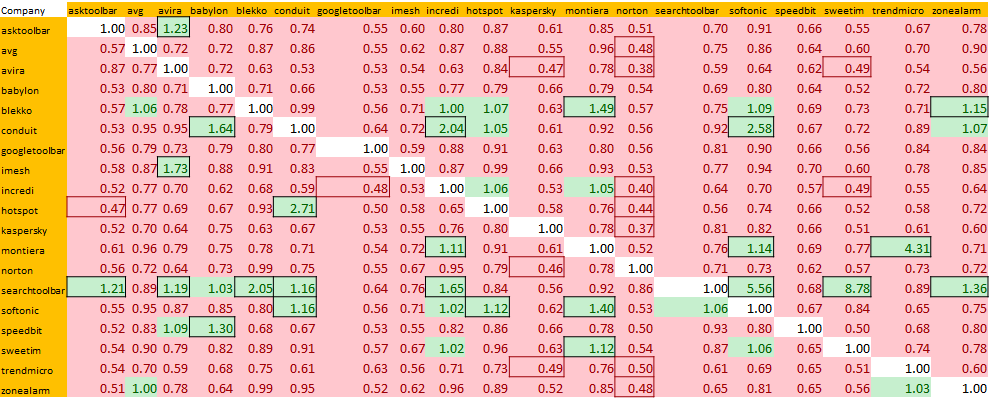
\includegraphics[scale=0.7]{figures/RatioMatrixPortrate1.png}
    \caption{Ratios of Expected PPR and expected PR scores of companies. Rows are companies in PPR queries.}
    \label{fig:RatioMatrix}
\end{figure}

Our methodology appears very successful in revealing truly symbiotic relations between companies. Below are a few examples. Their PPR to PR ratios can be seen in~\autoref{fig:RatioMatrix}, however we also show a separate figure per example.

In~\autoref{fig:incredi_sym_conduit}, we show the expected score of IncrediMail in Conduit's PPR and its expected score in non-personalized PageRank. We can see that IncrediMail's score increases significantly when PageRank is personalized around Conduit: as the personalized PageRank prioritizes Conduit, it also ``drags up'' IncrediMail. This implies that there is a close semantic relationship between Conduit and IncrediMail: as we mentioned in~\autoref{subsub:co_occurrence}, Conduit ended up merging with IncrediMail (which is now called Perion) in 2014. 

\begin{figure}[!htbp]
\centering
\begin{subfigure}[b]{0.4\textwidth}
	\centering
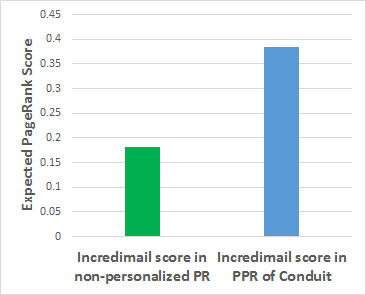
\includegraphics[width=\textwidth]{figures/incredi_sym_conduit1.png}
\caption{IncrediMail symbiotic relation with Conduit}
\label{fig:incredi_sym_conduit}
\end{subfigure}
\begin{subfigure}[b]{0.4\textwidth}
	\centering
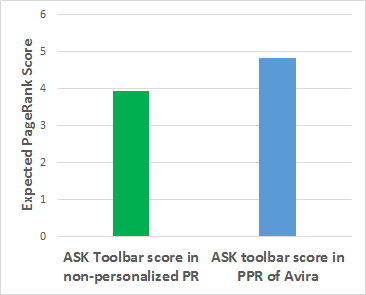
\includegraphics[width=\textwidth]{figures/ask_sym_avira.png}
\caption{ASK Toolbar symbiotic relation with Avira}
\label{fig:ask_sym_avira}
\end{subfigure}
\caption{Symbiotic relationship between companies}
	\label{fig:symbiotic_pagerank}
\end{figure}

%More symbiotic relations are shown in~\autoref{fig:symbiotic_2}. \autoref{fig:hotspot_sym_conduit} shows that HotSpot Shield is in symbiosis with Conduit, and this relationship can be verified in the Web\footnote{\url{https://www.pcrisk.com/removal-guides/7246-remove-hotspot-shield-toolbar}}.
\autoref{fig:ask_sym_avira} shows a rather unusual partnership between an antivirus company Avira and the addon distributor ASK. When investigating relationships between antivirus companies and addons distributors, we see that addon distributor scores usually suffer in PPRs of antivirus companies  (\autoref{fig:ask_clash_trend}). A simple explanation is that some browser addons are considered malware and are removed by antivirus products. Nevertheless, in \autoref{fig:ask_sym_avira}, we observe that ASK toolbar's score increases in Avira's PPR. An explanation can be found on Avira's official web site, which states that ``Avira chose Ask.com to be our partner in bringing you the SearchFree Toolbar $\dots$''\footnote{\url{https://www.avira.com/en/avira-searchfree-toolbar}}. 

The most interesting symbiotic relationships are those that cannot be validated in the Web. For example, SearchToolbar appears symbiotic with a few companies, with the highest PPR to PR score ratios for Softonic and SweetIM. SearchToolbar is manufactured by Zugo which is a small private company whose partnership agreements are not publicly disclosed. However, our results show that the existence of such agreements is quite apparent.

\subsection{Clash Relationships}
\label{sec:clash_relations}

In \autoref{sec:symb_relations}, we investigated symbiotic relationships between addon species, i.e. when one species benefit from another. In this section, we look for the opposite type of relationship: the \emph{clash}, which occurs when one species causes harm to another species. The idea behind detecting clash relations is very similar to the idea behind detecting simbiotic relations (as described in \autoref{sec:symb_relations}): we again aggregate addon PageRank scores into expected scores --- both for non-personalized PagerRank and personalized PageRank with a query of all company's addons. In contrast to looking for companies whose expected scores increase (which we assume correspond to symbiotic relations), we now look for companies whose scores decrease substantially when another company is in the PPR query. 


\begin{figure}[!htbp]
\centering
\begin{subfigure}[b]{0.4\textwidth}
	\centering
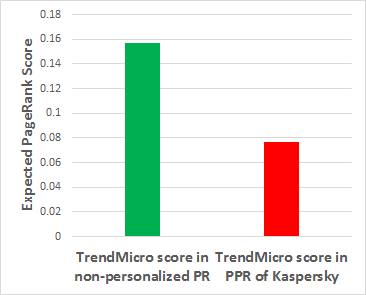
\includegraphics[width=\textwidth]{figures/trend_clash_kaspersky1.png}
\caption{TrendMicro clash relationship with Kaspersky}
\label{fig:trend_clash_kaspersky}
\end{subfigure}
\begin{subfigure}[b]{0.4\textwidth}
	\centering
%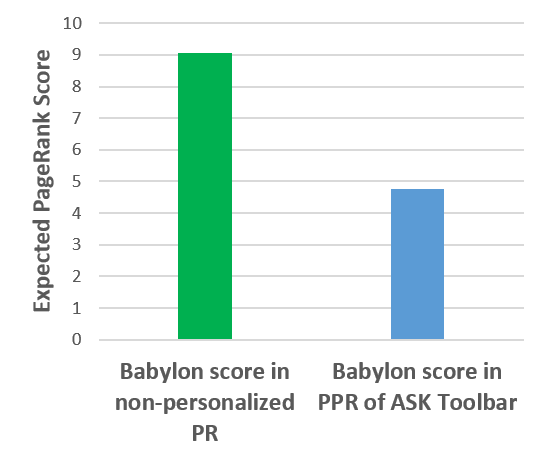
\includegraphics[width=\textwidth]{figures/babylon_nosym_ask.png}
%\caption{Babylon non-symbiotic relation with ASK}
%\label{fig:babylon_nosym_ask}
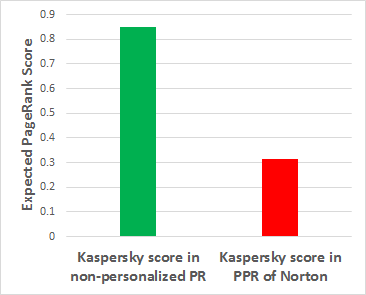
\includegraphics[width=\textwidth]{figures/kaspersky_clash_norton1.png}
\caption{Kaspersky clash relationship with Norton}
\label{fig:kaspersky_clash_norton}
\end{subfigure}
\caption{Clash relationship between antivirus companies}
	\label{fig:clash_av}
\end{figure}

As we can see in~\autoref{fig:RatioMatrix}, the company that experiences the most substantial plunge in the PPR to PR score ratios is Norton Antivirus. Other antivirus companies such as AVG, Avira, and Kaspersky clash strongly with Norton. A fairly straightforward validation of these results comes from the fact that there is a known competition between antivirus companies: in most cases, two antivirus software products cannot coexist on the same computer, so when one product gets installed the other often gets uninstalled. Norton is known for being preinstalled on many computers, while cheaper antivirus software such as AVG replaces Norton at a later stage. This is precisely the phenomenon we observe in our results. Two examples of clash relations in the antivirus domain are shown in \autoref{fig:clash_av}.

In the toolbar domain, it is remarkable to see that Google Toolbar appears clashing with all the other toolbars: smaller toolbar producers are likely to aim at uninstalling Google Toolbar as they consider Google their main competitor. \autoref{fig:ask_clash_trend} shows that when an antivirus company TrendMicro is in the query, it causes ASK Toolbar's scores to drop. Since antivirus companies sometimes treat toolbars as malware, this clash is not surprising. Another clash is shown in \autoref{fig:babylon_nosym_ask}, between ASK and Babylon (which are known rivals in the toolbar domain). Despite the fact that ASK and Babylon heavily co-occur in our dataset (see~\autoref{subsub:co_occurrence}), their clash is evident.

\begin{figure}[!htbp]
\centering
\begin{subfigure}[b]{0.4\textwidth}
	\centering
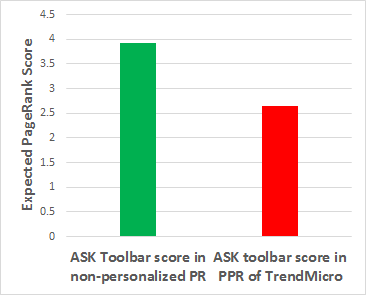
\includegraphics[width=\textwidth]{figures/ask_clash_trend1.png}
\caption{ASK Toolbar clash relation with TrendMicro}
\label{fig:ask_clash_trend}
\end{subfigure}
\begin{subfigure}[b]{0.4\textwidth}
	\centering
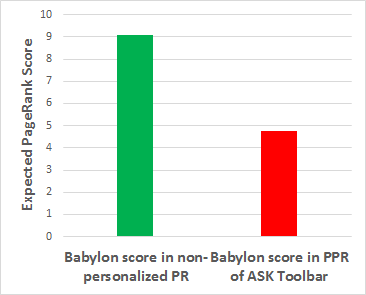
\includegraphics[width=\textwidth]{figures/babylon_nosym_ask1.png}
\caption{Babylon clash relation with ASK Toolbar}
%\caption{ASK Toolbar clash relation with TrendMicro}
\label{fig:babylon_nosym_ask}
\end{subfigure}
\caption{ASK Toolbar clash relations.}
	\label{fig:clash_1}
\end{figure}


\section{Summary}
\label{chap:summary}

The ecosystem of the Web browser is an unexplored research area. Thousands of browser addons fight their way to recognition and profitability. Addon manufacturers engage in partnerships or compete with each other. Most of this dynamics is hidden from the eyes of Web users. The goal of this work was to develop tools and methodologies for analyzing this complex ecosystem.

We were provided with a unique dataset of addons installed on almost a million machines. Initially, we tested numerous types of data representation, and applied a few machine learning algorithms, until we came up with the final decision about how to organize the data for future analysis. Our design choice is described in \autoref{sec:datasets}.

After organizing the data in a graph of users, addons, and terms extracted from addon attributes, we applied Personalized PageRank (PPR) to capture relationships between vertexes in the graph.

%Believing that user addons for some kind of an ecosystem with its own rules, we believed that since such rules exist we can conjectured that we can predict the addons behaviour.
First, we hypothesized that---analogously to a biological ecosystem---the Web browser ecosystem seeks to enter a steady state in which addons naturally coexist with each other. We looked for a way to verify our hypothesis by artificially ``disturbing'' the ecosystem and seeing whether it tends to come back to the steady state. Technically, we removed an edge between an addon node and the machine on which it was installed, and applied PPR to identify the missing edge. Given a query of all addons installed on a machine from which one addon got ``extracted'', our algorithm constructed a ranked list of addons most probable to be installed on that machine. We obtained impressive results: the extracted addon, with high probability, was found among the top 10 addons in the ranked list. In \autoref{chap:user_ecosystem}, we describe many experiments we conducted while searching for an optimal setup. Given the \emph{Big Data} size of the graph, we had to overcome technical difficulties in order to run many thousands of experiments in suitable amount of time. As the results show in \autoref{chap:user_ecosystem}, our approach significantly outperforms all the baselines.

While analyzing our results of \autoref{chap:user_ecosystem}, we observed some interesting phenomena: we saw that addons relate to each other not only via the machine they are installed on, but also via their manufacturing company. We saw that addons of some manufacturers appear more often with addons of other manufacturers, and do not appear with others.

Armed with this observation and with the methodology we developed in \autoref{chap:user_ecosystem}, we decided to explore this phenomena more deeply, and to shed light on the relations between addon manufactures. Our results are presented in \autoref{chap:Symbiosis}.
We discovered that some companies are engaged in \emph{symbiotic} relations---when one company's addons are installed on a machine, there is a good chance that another company's addons will be there too. We found out that a simple co-occurrence count is not good enough to detect symbiotic relations---most companies with high co-occurrence do not seem to be in symbiosis with each other. We applied PPR with all company's addons in the query and observed other company's addons improving their scores. Our methodology turned out being very effective at discovering symbiosis between companies---we managed to validate many symbiotic relations in online media. As a byproduct of this work, we created a method for mapping an addon to its manufacturing company, even if the addon's attributes provide no clue for this connection.

Building upon the success of discovering symbiosis, we applied the same methodology for discovering the opposite relation---we called it the \emph{clash} relation. In a PPR focused on a company's addons, we detected addons of another company dropping significantly their scores. Using this methodology, we discovered many clash relationships between companies, some of which could be easily validated online, while the others were hidden well enough such that our algorithm was the only one to discover them.

To summarize, we investigated a previously unexplored domain of the Web browser and the ecosystem of its addons. We showed that the Web browser ecosystem bears characteristics that closely---and surprisingly---resemble those of biological ecosystems. Addons behave very much like organisms, both at the local level of a single browser (in which subjects of different species co-exist and compete over the limited resource of the user's attention), and at the global level that reflects inter-species relationships. While the behavior of addon species is prescribed by their manufacturers---just like the behavior of many biological species is prescribed by the Nature---the local habitat of a specific browser develops autonomously with limited (or no) human intervention. It appears that the humanity just created a new class of organisms that, although being digital, behave much like biological. It is not hard to imagine that many other classes will come. While creating new digital organisms, the humanity seems to get prepared for the forthcoming Human-Computer Symbiosis.

\newpage
\phantomsection \label{Bibliography}
\addcontentsline{toc}{chapter}{Bibliography}
\bibliographystyle{ijocv081}
\bibliography{thesisdraft}

\end{document}


